\documentclass[12pt,aspectratio=169]{beamer}
\usepackage[T1]{fontenc}
\usepackage{lmodern,amsmath,amssymb,booktabs,tikz,graphicx}
\usetikzlibrary{arrows.meta,positioning,calc}
\definecolor{Ink}{HTML}{17324D}
\definecolor{Teal}{HTML}{007F7A}
\definecolor{Muted}{HTML}{556574}
\definecolor{Paper}{HTML}{FAFAF7}
\definecolor{Rust}{HTML}{AD532E}
\definecolor{Gold}{HTML}{B38630}
\setbeamercolor{background canvas}{bg=Paper}
\setbeamercolor{normal text}{fg=Ink}
\setbeamercolor{frametitle}{fg=Ink}
\setbeamercolor{structure}{fg=Teal}
\setbeamercolor{alerted text}{fg=Rust}
\setbeamerfont{frametitle}{size=\LARGE,series=\bfseries}
\setbeamertemplate{navigation symbols}{}
\setbeamersize{text margin left=9mm,text margin right=9mm}
\setbeamertemplate{frametitle}{\par\vspace{2mm}\insertframetitle\par\vspace{1mm}{\color{Gold}\rule{14mm}{1pt}}}
\setbeamertemplate{footline}{\hspace{9mm}\scriptsize\color{Muted}\insertsectionhead\hfill\insertframenumber\hspace{9mm}\vspace{4mm}}
\hypersetup{colorlinks=true,urlcolor=Teal,linkcolor=Muted,pdfauthor={}}
\newcommand{\point}[1]{\par\vspace{3mm}{\large #1\par}}
\newcommand{\eqnote}[1]{\par\vspace{2mm}{\small\color{Muted}#1\par}}
\newcommand{\smalltext}[1]{\eqnote{#1}}
\newcommand{\insight}[1]{\par\vspace{2mm}{\color{Teal}\bfseries #1}\par}
\newcommand{\identity}{\text{\scriptsize accounting identity}}
\newcommand{\policy}{R^{\mathrm{policy}}}
\newcommand{\loanrate}{R^{\mathrm{loan}}}
\newcommand{\nominal}{R^{\mathrm{nom}}}
\newcommand{\realrate}{R^{\mathrm{real}}}
\newcommand{\neutral}{R^{\mathrm{neutral}}}
\newcommand{\spot}[1]{R^{\mathrm{spot}}(#1)}
\newcommand{\forward}[2]{R^{\mathrm{forward}}(#1,#2)}
\newcommand{\bondyield}{R^{\mathrm{bond}}}
\newcommand{\bondrate}[1]{R^{\mathrm{bond}}(#1)}
\AtBeginDocument{\setlength{\abovedisplayskip}{5pt}\setlength{\belowdisplayskip}{5pt}\setlength{\abovedisplayshortskip}{3pt}\setlength{\belowdisplayshortskip}{3pt}}

\renewcommand{\policy}{\bar i}
\renewcommand{\nominal}{i}
\renewcommand{\loanrate}{i}
\renewcommand{\realrate}{r}
\renewcommand{\neutral}{r^\ast}
\usepackage{array}
\hypersetup{pdftitle={Economics and Finance for Mathematicians: Money, inflation and activity}}
\begin{document}

% Slide 1: Money, inflation and activity

\begin{frame}[plain]
{\color{Teal}\large ECONOMICS AND FINANCE\quad /\quad 02}\par\vspace{9mm}{\Huge\bfseries Money, inflation and activity}\par\vspace{7mm}{\Large How does a policy rate connect spending today to payments tomorrow?}
\end{frame}

% Slide 2: Short run and long run

\begin{frame}{Short run and long run}
\begin{center}\begin{tabular}{@{}>{\raggedright\arraybackslash}p{.45\textwidth}>{\raggedright\arraybackslash}p{.46\textwidth}@{}}\toprule \textbf{Short run} & \textbf{Long-run benchmark}\\\midrule Some prices and wages adjust slowly. & Prices and wages have adjusted.\\[2mm]
Demand can move output away from potential: $Y\ne Y^*$. & The output gap closes: $Y=Y^*$.\\[2mm]
Policy can change real borrowing costs and activity. & Real fundamentals shape the real interest rate.\\\bottomrule\end{tabular}\end{center}\eqnote{Purely nominal shocks mainly affect prices in the long-run benchmark. The horizon has no fixed calendar cutoff. Real shocks can move potential output itself.}
\end{frame}

% Slide 3: Money, production and spending

\begin{frame}[plain]
\begin{tikzpicture}[remember picture,overlay]
\node[inner sep=0] at (current page.center){
\includegraphics[width=\paperwidth,height=\paperheight]{assets/money_bakery.png}};
\fill[Paper] (current page.north west) rectangle ([yshift=-13mm]current page.north east);
\node[anchor=west,font=\Large\bfseries,text=Ink] at ([xshift=9mm,yshift=-6.5mm]current page.north west){Money, production and spending};
\fill[Paper] (current page.south west) rectangle ([yshift=13mm]current page.south east);
\node[anchor=west,text width=14.1cm,font=\small,text=Ink] at ([xshift=9mm,yshift=6.5mm]current page.south west){A loan can finance a new oven. Interest rates affect the investment decision.};
\end{tikzpicture}
\end{frame}

% Slide 4: Today’s route

\begin{frame}{Today’s route}
\point{Rates, purchasing power and the long-run real benchmark.}\point{Money demand and classic IS–LM with a fixed money supply.}\point{Inflation feedback, then modern rate targeting at the end.}
\end{frame}

% Slide 5: Interest and inflation
\section[Interest and inflation]{Interest and inflation}
\begin{frame}[plain]
{\color{Gold}\large LECTURE 2}\par\vspace{9mm}{\Huge\bfseries Interest and inflation}\par\vspace{7mm}{\Large What is the price of spending earlier?}
\end{frame}

% Slide 6: A zero-coupon bond exchanges money across time

\begin{frame}{A zero-coupon bond exchanges money across time}
\point{A zero-coupon bond makes one payment at maturity.}\[p_0=\frac{F}{(1+i)^T},\qquad F=100.\]\point{$p_0$: price today. $i$: annual nominal yield. $T$: years to maturity.}\[T=1,\quad i=5\%\quad\Rightarrow\quad p_0=\frac{100}{1.05}=95.24.\]
\end{frame}

% Slide 7: A higher yield means a lower bond price

\begin{frame}{A higher yield means a lower bond price}
\begin{center}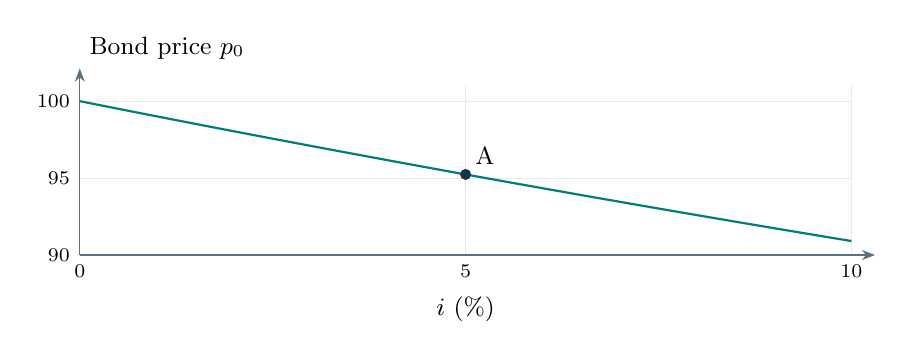
\begin{tikzpicture}[>=Stealth,every node/.style={font=\small}]
\draw[Ink!10] (0.0000,0.0000)--(0.0000,2.1500);\node[below,font=\scriptsize] at (0.0000,0.0000){0};
\draw[Ink!10] (4.9000,0.0000)--(4.9000,2.1500);\node[below,font=\scriptsize] at (4.9000,0.0000){5};
\draw[Ink!10] (9.8000,0.0000)--(9.8000,2.1500);\node[below,font=\scriptsize] at (9.8000,0.0000){10};
\draw[Ink!10] (0.0000,0.0000)--(9.8000,0.0000);\node[left,font=\scriptsize] at (0.0000,0.0000){90};
\draw[Ink!10] (0.0000,0.9773)--(9.8000,0.9773);\node[left,font=\scriptsize] at (0.0000,0.9773){95};
\draw[Ink!10] (0.0000,1.9545)--(9.8000,1.9545);\node[left,font=\scriptsize] at (0.0000,1.9545){100};
\draw[->,Ink!70] (0,0)--(10.100000000000001,0);\draw[->,Ink!70] (0,0)--(0,2.37);
\node[below] at (4.9,-.40){$i$ (\%)};\node[anchor=west] at (0,2.63){Bond price $p_0$};
\draw[Teal,thick] plot coordinates {(0.0000,1.9545) (0.0980,1.9350) (0.1960,1.9155) (0.2940,1.8961) (0.3920,1.8767) (0.4900,1.8573) (0.5880,1.8380) (0.6860,1.8187) (0.7840,1.7994) (0.8820,1.7802) (0.9800,1.7610) (1.0780,1.7419) (1.1760,1.7228) (1.2740,1.7037) (1.3720,1.6847) (1.4700,1.6657) (1.5680,1.6467) (1.6660,1.6278) (1.7640,1.6089) (1.8620,1.5901) (1.9600,1.5713) (2.0580,1.5525) (2.1560,1.5338) (2.2540,1.5151) (2.3520,1.4964) (2.4500,1.4778) (2.5480,1.4592) (2.6460,1.4407) (2.7440,1.4222) (2.8420,1.4037) (2.9400,1.3853) (3.0380,1.3669) (3.1360,1.3485) (3.2340,1.3302) (3.3320,1.3119) (3.4300,1.2936) (3.5280,1.2754) (3.6260,1.2572) (3.7240,1.2390) (3.8220,1.2209) (3.9200,1.2028) (4.0180,1.1847) (4.1160,1.1667) (4.2140,1.1487) (4.3120,1.1308) (4.4100,1.1129) (4.5080,1.0950) (4.6060,1.0771) (4.7040,1.0593) (4.8020,1.0416) (4.9000,1.0238) (4.9980,1.0061) (5.0960,0.9884) (5.1940,0.9708) (5.2920,0.9532) (5.3900,0.9356) (5.4880,0.9180) (5.5860,0.9005) (5.6840,0.8831) (5.7820,0.8656) (5.8800,0.8482) (5.9780,0.8308) (6.0760,0.8135) (6.1740,0.7962) (6.2720,0.7789) (6.3700,0.7616) (6.4680,0.7444) (6.5660,0.7272) (6.6640,0.7101) (6.7620,0.6930) (6.8600,0.6759) (6.9580,0.6588) (7.0560,0.6418) (7.1540,0.6248) (7.2520,0.6078) (7.3500,0.5909) (7.4480,0.5740) (7.5460,0.5571) (7.6440,0.5403) (7.7420,0.5235) (7.8400,0.5067) (7.9380,0.4900) (8.0360,0.4733) (8.1340,0.4566) (8.2320,0.4400) (8.3300,0.4233) (8.4280,0.4067) (8.5260,0.3902) (8.6240,0.3737) (8.7220,0.3572) (8.8200,0.3407) (8.9180,0.3243) (9.0160,0.3079) (9.1140,0.2915) (9.2120,0.2751) (9.3100,0.2588) (9.4080,0.2425) (9.5060,0.2263) (9.6040,0.2101) (9.7020,0.1939) (9.8000,0.1777)};
\fill[Ink] (4.9000,1.0238) circle (2pt);\node[above right] at (4.9000,1.0238){A};
\end{tikzpicture}\end{center}\[\frac{\partial p_0}{\partial i}=-\frac{TF}{(1+i)^{T+1}}<0.\]\eqnote{With face value 100, a one-year price falls from 95.24 at 5\% to 90.91 at 10\%.}
\end{frame}

% Slide 8: Three rate symbols are enough

\begin{frame}{Three rate symbols are enough}
\begin{center}\begin{tabular}{@{}ll@{}}\toprule \textbf{Symbol} & \textbf{Meaning}\\\midrule $i$ & Nominal interest rate\\[2mm]
$\bar i$ & Central bank’s chosen policy-rate target\\[2mm]
$r$ & Real interest rate, measured in purchasing power\\\bottomrule\end{tabular}\end{center}\eqnote{Each rate has a stated horizon. In the classic IS–LM model, i is a market outcome.}
\end{frame}

% Slide 9: A real return measures purchasing power

\begin{frame}{A real return measures purchasing power}
\point{Nominal return counts money. Real return counts what it buys.}\[1+r^{\rm realised}_{t+1}=\frac{1+i_t}{1+\pi_{t+1}}.\]\eqnote{Exact purchasing-power conversion: return and realised inflation cover the same period.}
\end{frame}

% Slide 10: The Fisher approximation comes from logarithms

\begin{frame}{The Fisher approximation comes from logarithms}
\[\ln(1+r)=\ln(1+i)-\ln(1+\pi).\]\point{For small rates, $\ln(1+x)\approx x$.}\[\boxed{r\approx i-\pi.}\]\eqnote{Exact in log gross rates; approximate in simple percentage rates. This line uses realised inflation.}
\end{frame}

% Slide 11: For decisions today, expected inflation matters

\begin{frame}{For decisions today, expected inflation matters}
\[\boxed{r_t\approx i_t-\pi_t^e,\qquad\pi_t^e\equiv\mathbb E_t\pi_{t+1}.}\]\point{$\pi_t^e$: expected inflation over the investment horizon.}\[i_t=5\%,\quad\pi_t^e=3\%\quad\Rightarrow\quad r_t\approx2\%.\]\eqnote{From here, r denotes the approximate expected real rate relevant for decisions.}
\end{frame}

% Slide 12: A nominal cut need not reduce the real rate

\begin{frame}{A nominal cut need not reduce the real rate}
\begin{center}\begin{tabular}{@{}lll@{}}\toprule \textbf{} & \textbf{Before} & \textbf{After}\\\midrule Nominal rate $\nominal$ & 5\% & 4\%\\[2mm]
Expected inflation & 3\% & 1\%\\[2mm]
Approximate real rate $\realrate$ & 2\% & 3\%\\\bottomrule\end{tabular}\end{center}\point{Expected inflation fell faster than the nominal rate.}
\end{frame}

% Slide 13: Saving, investment and the real rate

\begin{frame}{Saving, investment and the real rate}
\begin{center}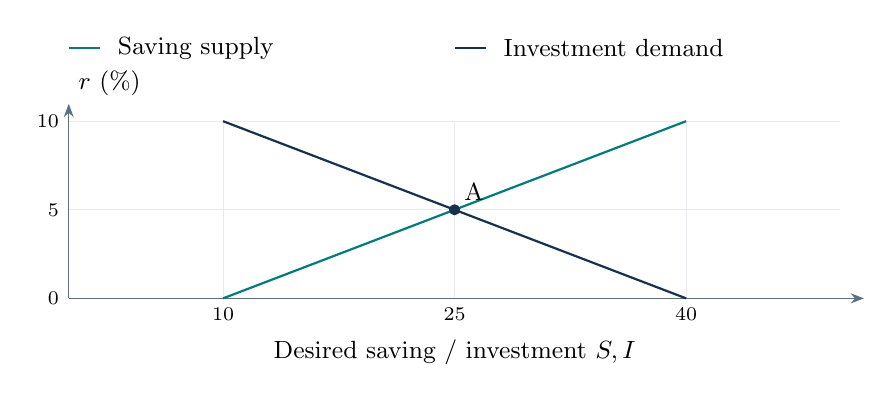
\begin{tikzpicture}[>=Stealth,every node/.style={font=\small}]
\draw[Ink!10] (1.9600,0.0000)--(1.9600,2.2500);\node[below,font=\scriptsize] at (1.9600,0.0000){10};
\draw[Ink!10] (4.9000,0.0000)--(4.9000,2.2500);\node[below,font=\scriptsize] at (4.9000,0.0000){25};
\draw[Ink!10] (7.8400,0.0000)--(7.8400,2.2500);\node[below,font=\scriptsize] at (7.8400,0.0000){40};
\draw[Ink!10] (0.0000,0.0000)--(9.8000,0.0000);\node[left,font=\scriptsize] at (0.0000,0.0000){0};
\draw[Ink!10] (0.0000,1.1250)--(9.8000,1.1250);\node[left,font=\scriptsize] at (0.0000,1.1250){5};
\draw[Ink!10] (0.0000,2.2500)--(9.8000,2.2500);\node[left,font=\scriptsize] at (0.0000,2.2500){10};
\draw[->,Ink!70] (0,0)--(10.100000000000001,0);\draw[->,Ink!70] (0,0)--(0,2.47);
\node[below] at (4.9,-.40){Desired saving / investment $S,I$};\node[anchor=west] at (0,2.73){$r$ (\%)};
\draw[Teal,thick] plot coordinates {(1.9600,0.0000) (7.8400,2.2500)};
\draw[Ink,thick] plot coordinates {(7.8400,0.0000) (1.9600,2.2500)};
\fill[Ink] (4.9000,1.1250) circle (2pt);\node[above right] at (4.9000,1.1250){A};
\draw[Teal,thick] (0.0,3.18)--(0.4,3.18);\node[anchor=west,font=\small] at (0.5,3.18){Saving supply};
\draw[Ink,thick] (4.9,3.18)--(5.300000000000001,3.18);\node[anchor=west,font=\small] at (5.4,3.18){Investment demand};
\end{tikzpicture}\end{center}\eqnote{At A: planned saving and investment both equal 25; r = 5\%. Hypothetical units.}
\end{frame}

% Slide 14: A larger harvest can lower the real rate

\begin{frame}{A larger harvest can lower the real rate}
\begin{center}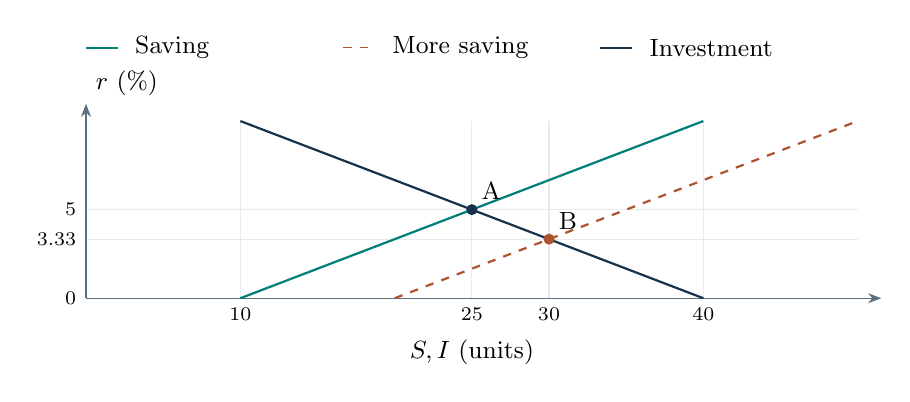
\begin{tikzpicture}[>=Stealth,every node/.style={font=\small}]
\draw[Ink!10] (1.9600,0.0000)--(1.9600,2.2500);\node[below,font=\scriptsize] at (1.9600,0.0000){10};
\draw[Ink!10] (4.9000,0.0000)--(4.9000,2.2500);\node[below,font=\scriptsize] at (4.9000,0.0000){25};
\draw[Ink!10] (5.8800,0.0000)--(5.8800,2.2500);\node[below,font=\scriptsize] at (5.8800,0.0000){30};
\draw[Ink!10] (7.8400,0.0000)--(7.8400,2.2500);\node[below,font=\scriptsize] at (7.8400,0.0000){40};
\draw[Ink!10] (0.0000,0.0000)--(9.8000,0.0000);\node[left,font=\scriptsize] at (0.0000,0.0000){0};
\draw[Ink!10] (0.0000,0.7500)--(9.8000,0.7500);\node[left,font=\scriptsize] at (0.0000,0.7500){3.33};
\draw[Ink!10] (0.0000,1.1250)--(9.8000,1.1250);\node[left,font=\scriptsize] at (0.0000,1.1250){5};
\draw[->,Ink!70] (0,0)--(10.100000000000001,0);\draw[->,Ink!70] (0,0)--(0,2.47);
\node[below] at (4.9,-.40){$S,I$ (units)};\node[anchor=west] at (0,2.73){$r$ (\%)};
\draw[Teal,thick] plot coordinates {(1.9600,0.0000) (7.8400,2.2500)};
\draw[Rust,dashed,thick] plot coordinates {(3.9200,0.0000) (9.8000,2.2500)};
\draw[Ink,thick] plot coordinates {(7.8400,0.0000) (1.9600,2.2500)};
\fill[Ink] (4.9000,1.1250) circle (2pt);\node[above right] at (4.9000,1.1250){A};
\fill[Rust] (5.8800,0.7500) circle (2pt);\node[above right] at (5.8800,0.7500){B};
\draw[Teal,thick] (0.0,3.18)--(0.4,3.18);\node[anchor=west,font=\small] at (0.5,3.18){Saving};
\draw[Rust,dashed] (3.266666666666667,3.18)--(3.666666666666667,3.18);\node[anchor=west,font=\small] at (3.766666666666667,3.18){More saving};
\draw[Ink,thick] (6.533333333333334,3.18)--(6.9333333333333345,3.18);\node[anchor=west,font=\small] at (7.033333333333334,3.18){Investment};
\end{tikzpicture}\end{center}\eqnote{Extra income raises saving supply by 10. The real rate falls from 5\% to 3.33\%.}
\end{frame}

% Slide 15: Better projects can raise the real rate

\begin{frame}{Better projects can raise the real rate}
\begin{center}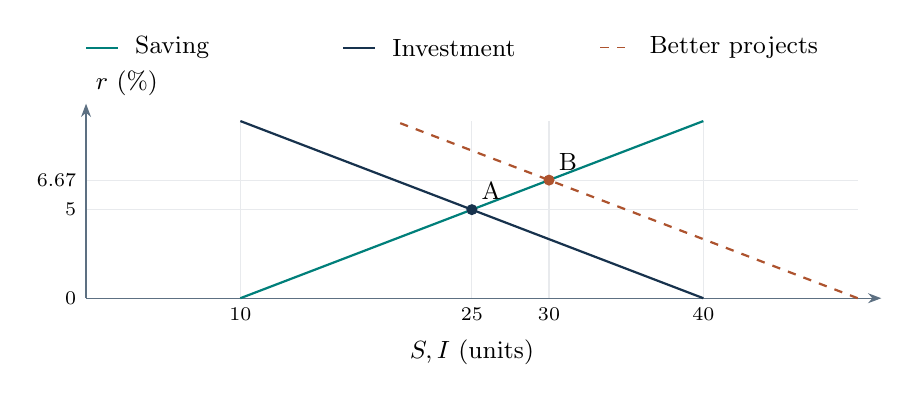
\begin{tikzpicture}[>=Stealth,every node/.style={font=\small}]
\draw[Ink!10] (1.9600,0.0000)--(1.9600,2.2500);\node[below,font=\scriptsize] at (1.9600,0.0000){10};
\draw[Ink!10] (4.9000,0.0000)--(4.9000,2.2500);\node[below,font=\scriptsize] at (4.9000,0.0000){25};
\draw[Ink!10] (5.8800,0.0000)--(5.8800,2.2500);\node[below,font=\scriptsize] at (5.8800,0.0000){30};
\draw[Ink!10] (7.8400,0.0000)--(7.8400,2.2500);\node[below,font=\scriptsize] at (7.8400,0.0000){40};
\draw[Ink!10] (0.0000,0.0000)--(9.8000,0.0000);\node[left,font=\scriptsize] at (0.0000,0.0000){0};
\draw[Ink!10] (0.0000,1.1250)--(9.8000,1.1250);\node[left,font=\scriptsize] at (0.0000,1.1250){5};
\draw[Ink!10] (0.0000,1.5000)--(9.8000,1.5000);\node[left,font=\scriptsize] at (0.0000,1.5000){6.67};
\draw[->,Ink!70] (0,0)--(10.100000000000001,0);\draw[->,Ink!70] (0,0)--(0,2.47);
\node[below] at (4.9,-.40){$S,I$ (units)};\node[anchor=west] at (0,2.73){$r$ (\%)};
\draw[Teal,thick] plot coordinates {(1.9600,0.0000) (7.8400,2.2500)};
\draw[Ink,thick] plot coordinates {(7.8400,0.0000) (1.9600,2.2500)};
\draw[Rust,dashed,thick] plot coordinates {(9.8000,0.0000) (3.9200,2.2500)};
\fill[Ink] (4.9000,1.1250) circle (2pt);\node[above right] at (4.9000,1.1250){A};
\fill[Rust] (5.8800,1.5000) circle (2pt);\node[above right] at (5.8800,1.5000){B};
\draw[Teal,thick] (0.0,3.18)--(0.4,3.18);\node[anchor=west,font=\small] at (0.5,3.18){Saving};
\draw[Ink,thick] (3.266666666666667,3.18)--(3.666666666666667,3.18);\node[anchor=west,font=\small] at (3.766666666666667,3.18){Investment};
\draw[Rust,dashed] (6.533333333333334,3.18)--(6.9333333333333345,3.18);\node[anchor=west,font=\small] at (7.033333333333334,3.18){Better projects};
\end{tikzpicture}\end{center}\eqnote{Firms want 10 more units at each rate. Competition for resources raises r from 5\% to 6.67\%.}
\end{frame}

% Slide 16: The long-run Fisher effect

\begin{frame}{The long-run Fisher effect}
\begin{center}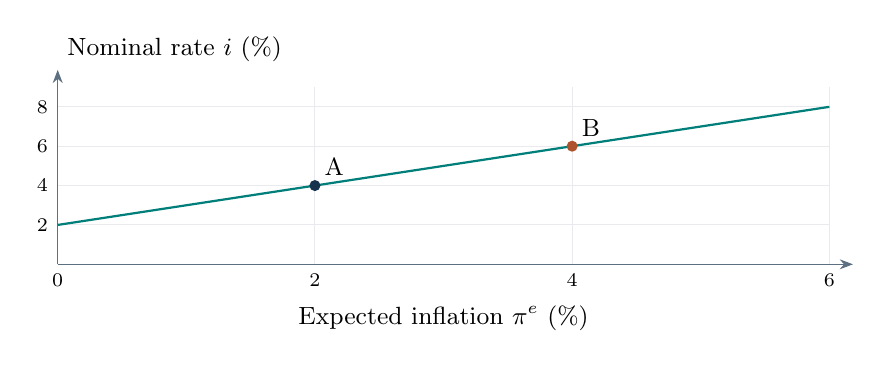
\begin{tikzpicture}[>=Stealth,every node/.style={font=\small}]
\draw[Ink!10] (0.0000,0.0000)--(0.0000,2.2500);\node[below,font=\scriptsize] at (0.0000,0.0000){0};
\draw[Ink!10] (3.2667,0.0000)--(3.2667,2.2500);\node[below,font=\scriptsize] at (3.2667,0.0000){2};
\draw[Ink!10] (6.5333,0.0000)--(6.5333,2.2500);\node[below,font=\scriptsize] at (6.5333,0.0000){4};
\draw[Ink!10] (9.8000,0.0000)--(9.8000,2.2500);\node[below,font=\scriptsize] at (9.8000,0.0000){6};
\draw[Ink!10] (0.0000,0.5000)--(9.8000,0.5000);\node[left,font=\scriptsize] at (0.0000,0.5000){2};
\draw[Ink!10] (0.0000,1.0000)--(9.8000,1.0000);\node[left,font=\scriptsize] at (0.0000,1.0000){4};
\draw[Ink!10] (0.0000,1.5000)--(9.8000,1.5000);\node[left,font=\scriptsize] at (0.0000,1.5000){6};
\draw[Ink!10] (0.0000,2.0000)--(9.8000,2.0000);\node[left,font=\scriptsize] at (0.0000,2.0000){8};
\draw[->,Ink!70] (0,0)--(10.100000000000001,0);\draw[->,Ink!70] (0,0)--(0,2.47);
\node[below] at (4.9,-.40){Expected inflation $\pi^e$ (\%)};\node[anchor=west] at (0,2.73){Nominal rate $i$ (\%)};
\draw[Teal,thick] plot coordinates {(0.0000,0.5000) (9.8000,2.0000)};
\fill[Ink] (3.2667,1.0000) circle (2pt);\node[above right] at (3.2667,1.0000){A};
\fill[Rust] (6.5333,1.5000) circle (2pt);\node[above right] at (6.5333,1.5000){B};
\end{tikzpicture}\end{center}\[i\approx r^*+\pi^e,\qquad r^*=2\%\text{ held fixed}.\]\eqnote{With r* fixed, expected inflation and the nominal rate both rise by about 2 points.}
\end{frame}

% Slide 17: The causal story depends on the horizon

\begin{frame}{The causal story depends on the horizon}
\begin{center}\begin{tabular}{@{}p{.46\textwidth}p{.46\textwidth}@{}}\toprule \textbf{Long-run benchmark} & \textbf{Short-run experiment}\\\midrule Resources, tastes and technology pin down the real benchmark. & Sticky prices and expectations can adjust slowly.\\[2mm]
$r=r^*,\quad i\approx r^*+\pi^e$. & Policy changes $\bar i$; then $r\approx\bar i-\pi^e$ changes.\\\bottomrule\end{tabular}\end{center}\eqnote{A higher nominal rate can reflect higher expected inflation or tighter real restraint. Specify the experiment.}
\end{frame}

% Slide 18: Inflation measures a change in the price level

\begin{frame}{Inflation measures a change in the price level}
\point{$P_t$: the cost index of a representative basket.}\[\pi_t=\frac{P_t-P_{t-1}}{P_{t-1}}.\]\point{Inflation means the same money buys less of that basket.}\eqnote{Where does the extra money for higher prices come from? The next example needs none.}
\end{frame}

% Slide 19: Prices can rise without any extra money

\begin{frame}{Prices can rise without any extra money}
\begin{center}\begin{tabular}{@{}lll@{}}\toprule \textbf{One-good economy, one period} & \textbf{Before} & \textbf{Supply shortfall}\\\midrule Money spent in the period & 100 & 100\\[2mm]
Goods available & 10 & 5\\[2mm]
Price per good & 10 & 20\\\bottomrule\end{tabular}\end{center}\point{The same spending competes for fewer goods.}\eqnote{Fixed nominal spending and no extra money in this hypothetical example.}
\end{frame}

% Slide 20: New money and faster spending are other possibilities

\begin{frame}{New money and faster spending are other possibilities}
\[MV=PY,\qquad V\equiv\frac{PY}{M}.\]\point{Bank lending can create new deposits.}\point{Existing balances can circulate faster: the same money supports more spending.}\eqnote{M is a money stock; PY is nominal output over a period; V is its turnover ratio.}
\end{frame}

% Slide 21: Disinflation can leave prices higher

\begin{frame}{Disinflation can leave prices higher}
\begin{center}\begin{tabular}{@{}lll@{}}\toprule \textbf{Date} & \textbf{Basket price} & \textbf{Inflation}\\\midrule 0 & 100 & --\\[2mm]
1 & 110 & 10\%\\[2mm]
2 & 112.20 & 2\%\\\bottomrule\end{tabular}\end{center}\point{Inflation fell. The price level continued to rise.}
\end{frame}

% Slide 22: Demand pressure can raise prices

\begin{frame}{Demand pressure can raise prices}
\point{Orders grow faster than firms can expand production.}\par\vspace{4mm}\begin{center}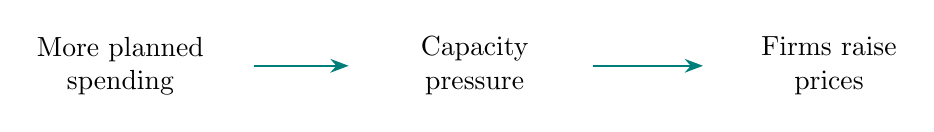
\begin{tikzpicture}[>=Stealth,every node/.style={align=center}] \node at (0,0){More planned\\spending};\node at (4.5,0){Capacity\\pressure};\node at (9,0){Firms raise\\prices}; \draw[->,Teal,thick](1.7,0)--(2.9,0);\draw[->,Teal,thick](6,0)--(7.4,0);\end{tikzpicture}\end{center}\point{The effect depends on how much productive slack remains.}
\end{frame}

% Slide 23: Supply shocks can raise prices while output weakens

\begin{frame}{Supply shocks can raise prices while output weakens}
\point{An energy shortage makes production more expensive.}\point{Firms may raise prices and produce less at the same time.}\eqnote{A central bank can influence demand. It cannot create the missing energy.}
\end{frame}

% Slide 24: Expectations can make inflation persistent

\begin{frame}{Expectations can make inflation persistent}
\point{Expected cost increases enter wage negotiations and pricing plans.}\point{Contracts can carry an initial shock into later periods.}\eqnote{Wage catch-up alone does not establish an explosive wage-price spiral.}
\end{frame}

% Slide 25: Why high or volatile inflation is costly

\begin{frame}{Why high or volatile inflation is costly}
\point{Unindexed income and savings lose purchasing power.}\point{Unexpected inflation redistributes value in nominal contracts.}\point{Unstable prices make planning and relative-price signals harder.}
\end{frame}

% Slide 26: Why choose a small positive target?

\begin{frame}{Why choose a small positive target?}
\point{A buffer against persistent deflation.}\point{More room to lower real rates when nominal rates face a lower bound.}\point{Easier real-wage adjustment when nominal wages are sticky.}\eqnote{The ECB targets 2\% inflation over the medium term. This is a policy choice.}
\end{frame}

% Slide 27: Constant inflation compounds the price level

\begin{frame}{Constant inflation compounds the price level}
\begin{center}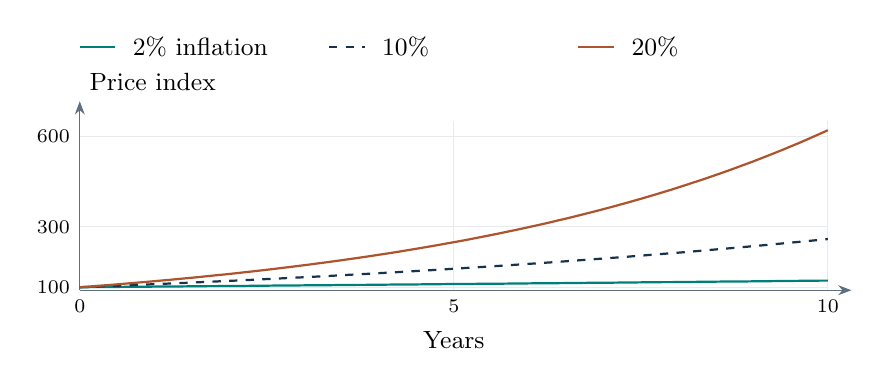
\begin{tikzpicture}[>=Stealth,every node/.style={font=\small}]
\draw[Ink!10] (0.000,0.000)--(0.000,2.150);\node[below,font=\scriptsize] at (0.000,0.000){0};
\draw[Ink!10] (4.750,0.000)--(4.750,2.150);\node[below,font=\scriptsize] at (4.750,0.000){5};
\draw[Ink!10] (9.500,0.000)--(9.500,2.150);\node[below,font=\scriptsize] at (9.500,0.000){10};
\draw[Ink!10] (0.000,0.038)--(9.500,0.038);\node[left,font=\scriptsize] at (0.000,0.038){100};
\draw[Ink!10] (0.000,0.806)--(9.500,0.806);\node[left,font=\scriptsize] at (0.000,0.806){300};
\draw[Ink!10] (0.000,1.958)--(9.500,1.958);\node[left,font=\scriptsize] at (0.000,1.958){600};
\draw[->,Ink!70] (0,0)--(9.8,0);\draw[->,Ink!70] (0,0)--(0,2.4);
\node[below] at (4.75,-.40){Years};\node[anchor=west] at (0,2.65){Price index};
\draw[Teal,thick] plot coordinates {(0.000,0.038) (0.095,0.039) (0.190,0.040) (0.285,0.041) (0.380,0.041) (0.475,0.042) (0.570,0.043) (0.665,0.044) (0.760,0.045) (0.855,0.045) (0.950,0.046) (1.045,0.047) (1.140,0.048) (1.235,0.048) (1.330,0.049) (1.425,0.050) (1.520,0.051) (1.615,0.052) (1.710,0.052) (1.805,0.053) (1.900,0.054) (1.995,0.055) (2.090,0.055) (2.185,0.056) (2.280,0.057) (2.375,0.058) (2.470,0.059) (2.565,0.059) (2.660,0.060) (2.755,0.061) (2.850,0.062) (2.945,0.063) (3.040,0.064) (3.135,0.064) (3.230,0.065) (3.325,0.066) (3.420,0.067) (3.515,0.068) (3.610,0.068) (3.705,0.069) (3.800,0.070) (3.895,0.071) (3.990,0.072) (4.085,0.073) (4.180,0.073) (4.275,0.074) (4.370,0.075) (4.465,0.076) (4.560,0.077) (4.655,0.078) (4.750,0.078) (4.845,0.079) (4.940,0.080) (5.035,0.081) (5.130,0.082) (5.225,0.083) (5.320,0.083) (5.415,0.084) (5.510,0.085) (5.605,0.086) (5.700,0.087) (5.795,0.088) (5.890,0.089) (5.985,0.089) (6.080,0.090) (6.175,0.091) (6.270,0.092) (6.365,0.093) (6.460,0.094) (6.555,0.095) (6.650,0.095) (6.745,0.096) (6.840,0.097) (6.935,0.098) (7.030,0.099) (7.125,0.100) (7.220,0.101) (7.315,0.102) (7.410,0.103) (7.505,0.103) (7.600,0.104) (7.695,0.105) (7.790,0.106) (7.885,0.107) (7.980,0.108) (8.075,0.109) (8.170,0.110) (8.265,0.111) (8.360,0.111) (8.455,0.112) (8.550,0.113) (8.645,0.114) (8.740,0.115) (8.835,0.116) (8.930,0.117) (9.025,0.118) (9.120,0.119) (9.215,0.120) (9.310,0.121) (9.405,0.122) (9.500,0.122)};
\draw[Ink,thick,dashed] plot coordinates {(0.000,0.038) (0.095,0.042) (0.190,0.046) (0.285,0.050) (0.380,0.053) (0.475,0.057) (0.570,0.061) (0.665,0.065) (0.760,0.069) (0.855,0.073) (0.950,0.077) (1.045,0.081) (1.140,0.085) (1.235,0.089) (1.330,0.093) (1.425,0.097) (1.520,0.102) (1.615,0.106) (1.710,0.110) (1.805,0.115) (1.900,0.119) (1.995,0.123) (2.090,0.128) (2.185,0.132) (2.280,0.137) (2.375,0.142) (2.470,0.146) (2.565,0.151) (2.660,0.156) (2.755,0.161) (2.850,0.165) (2.945,0.170) (3.040,0.175) (3.135,0.180) (3.230,0.185) (3.325,0.190) (3.420,0.196) (3.515,0.201) (3.610,0.206) (3.705,0.211) (3.800,0.217) (3.895,0.222) (3.990,0.227) (4.085,0.233) (4.180,0.238) (4.275,0.244) (4.370,0.250) (4.465,0.255) (4.560,0.261) (4.655,0.267) (4.750,0.273) (4.845,0.279) (4.940,0.285) (5.035,0.291) (5.130,0.297) (5.225,0.303) (5.320,0.309) (5.415,0.315) (5.510,0.322) (5.605,0.328) (5.700,0.335) (5.795,0.341) (5.890,0.348) (5.985,0.354) (6.080,0.361) (6.175,0.368) (6.270,0.375) (6.365,0.382) (6.460,0.389) (6.555,0.396) (6.650,0.403) (6.745,0.410) (6.840,0.417) (6.935,0.424) (7.030,0.432) (7.125,0.439) (7.220,0.447) (7.315,0.454) (7.410,0.462) (7.505,0.470) (7.600,0.477) (7.695,0.485) (7.790,0.493) (7.885,0.501) (7.980,0.509) (8.075,0.518) (8.170,0.526) (8.265,0.534) (8.360,0.543) (8.455,0.551) (8.550,0.560) (8.645,0.568) (8.740,0.577) (8.835,0.586) (8.930,0.595) (9.025,0.604) (9.120,0.613) (9.215,0.622) (9.310,0.631) (9.405,0.641) (9.500,0.650)};
\draw[Rust,thick] plot coordinates {(0.000,0.038) (0.095,0.045) (0.190,0.053) (0.285,0.060) (0.380,0.067) (0.475,0.075) (0.570,0.083) (0.665,0.091) (0.760,0.099) (0.855,0.107) (0.950,0.115) (1.045,0.124) (1.140,0.132) (1.235,0.141) (1.330,0.150) (1.425,0.159) (1.520,0.168) (1.615,0.178) (1.710,0.188) (1.805,0.197) (1.900,0.207) (1.995,0.217) (2.090,0.228) (2.185,0.238) (2.280,0.249) (2.375,0.260) (2.470,0.271) (2.565,0.283) (2.660,0.294) (2.755,0.306) (2.850,0.318) (2.945,0.330) (3.040,0.343) (3.135,0.355) (3.230,0.368) (3.325,0.381) (3.420,0.395) (3.515,0.408) (3.610,0.422) (3.705,0.436) (3.800,0.451) (3.895,0.465) (3.990,0.480) (4.085,0.495) (4.180,0.511) (4.275,0.527) (4.370,0.543) (4.465,0.559) (4.560,0.576) (4.655,0.593) (4.750,0.610) (4.845,0.627) (4.940,0.645) (5.035,0.664) (5.130,0.682) (5.225,0.701) (5.320,0.720) (5.415,0.740) (5.510,0.760) (5.605,0.780) (5.700,0.801) (5.795,0.822) (5.890,0.843) (5.985,0.865) (6.080,0.888) (6.175,0.910) (6.270,0.933) (6.365,0.957) (6.460,0.981) (6.555,1.005) (6.650,1.030) (6.745,1.055) (6.840,1.081) (6.935,1.107) (7.030,1.134) (7.125,1.161) (7.220,1.189) (7.315,1.217) (7.410,1.246) (7.505,1.275) (7.600,1.305) (7.695,1.336) (7.790,1.367) (7.885,1.398) (7.980,1.430) (8.075,1.463) (8.170,1.496) (8.265,1.530) (8.360,1.565) (8.455,1.600) (8.550,1.635) (8.645,1.672) (8.740,1.709) (8.835,1.747) (8.930,1.785) (9.025,1.825) (9.120,1.864) (9.215,1.905) (9.310,1.947) (9.405,1.989) (9.500,2.032)};
\draw[Teal,thick] (0.0,3.09)--(0.45,3.09);\node[anchor=west,font=\small] at (0.55,3.09){2\% inflation};
\draw[Ink,thick,dashed] (3.1666666666666665,3.09)--(3.6166666666666667,3.09);\node[anchor=west,font=\small] at (3.716666666666667,3.09){10\%};
\draw[Rust,thick] (6.333333333333333,3.09)--(6.783333333333333,3.09);\node[anchor=west,font=\small] at (6.883333333333333,3.09){20\%};

\end{tikzpicture}\end{center}\[P_t=P_0(1+\pi)^t.\]
\end{frame}

% Slide 28: Money and short rates
\section[Money and short rates]{Money and short rates}
\begin{frame}[plain]
{\color{Gold}\large LECTURE 2}\par\vspace{9mm}{\Huge\bfseries Money and short rates}\par\vspace{7mm}{\Large What can a central bank actually change?}
\end{frame}

% Slide 29: A bank loan creates an asset and a deposit

\begin{frame}{A bank loan creates an asset and a deposit}
\begin{center}\begin{tabular}{@{}ll@{}}\toprule \textbf{Bank assets} & \textbf{Bank liabilities}\\\midrule Loan to borrower: +100 & Borrower's deposit: +100\\\bottomrule\end{tabular}\end{center}\point{The borrower receives spendable money and an equal debt.}\eqnote{Lending still faces credit, capital, funding and liquidity constraints.}
\end{frame}

% Slide 30: The central bank anchors short-term market rates

\begin{frame}{The central bank anchors short-term market rates}
\point{Banks use central-bank reserves to settle payments.}\point{Administered rates and operations implement the overnight target $\bar i$.}\eqnote{Long yields also depend on expected future policy and risk premia. Exceptional regimes target them directly.}
\end{frame}

% Slide 31: Exception: a central bank can target a long yield

\begin{frame}{Exception: a central bank can target a long yield}
\point{In 2016, the BoJ introduced yield curve control.}\point{It bought Japanese government bonds to keep the ten-year yield around 0\%.}\[p_0=\frac{100}{(1+i)^T}:\quad\text{support the bond price to restrain its yield}.\]\eqnote{A historical policy example. The ZCB formula illustrates the price/yield mechanism.}
\end{frame}

% Slide 32: Money is useful, but costly to hold

\begin{frame}{Money is useful, but costly to hold}
\point{Money settles purchases and provides liquidity.}\point{Holding it can give up interest on an alternative asset.}
\end{frame}

% Slide 33: Real money balances measure purchasing power

\begin{frame}{Real money balances measure purchasing power}
\[\text{Real balances}=\frac{M}{P}.\]\begin{center}\begin{tabular}{@{}lll@{}}\toprule \textbf{A representative basket} & \textbf{Before} & \textbf{Prices double}\\\midrule Nominal money M & 100 & 100\\[2mm]
Price P per basket & 10 & 20\\[2mm]
Baskets the balance can buy & 10 & 5\\\bottomrule\end{tabular}\end{center}\eqnote{M/P is purchasing power held for transactions, measured as a stock.}
\end{frame}

% Slide 34: The money-market condition

\begin{frame}{The money-market condition}
\[\boxed{\frac{M}{P}=L(Y,i),\qquad L_Y>0,\quad L_i<0.}\]\begin{center}\begin{tabular}{@{}ll@{}}\toprule \textbf{Symbol} & \textbf{Meaning}\\\midrule M & Nominal money stock chosen in the classic model\\[2mm]
P & Price level, fixed in this experiment\\[2mm]
L(Y,i) & Desired real money holdings\\\bottomrule\end{tabular}\end{center}\eqnote{More real transactions raise money demand. Higher bond interest makes cash more costly to hold.}
\end{frame}

% Slide 35: The money-demand diagram

\begin{frame}{The money-demand diagram}
\begin{center}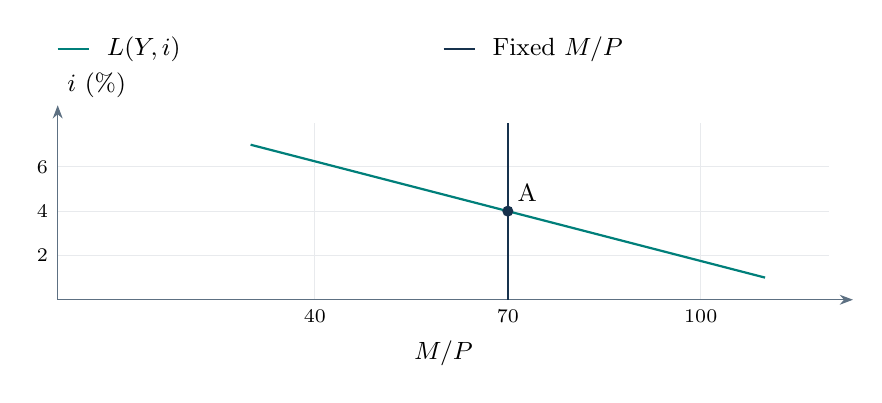
\begin{tikzpicture}[>=Stealth,every node/.style={font=\small}]
\draw[Ink!10] (3.2667,0.0000)--(3.2667,2.2500);\node[below,font=\scriptsize] at (3.2667,0.0000){40};
\draw[Ink!10] (5.7167,0.0000)--(5.7167,2.2500);\node[below,font=\scriptsize] at (5.7167,0.0000){70};
\draw[Ink!10] (8.1667,0.0000)--(8.1667,2.2500);\node[below,font=\scriptsize] at (8.1667,0.0000){100};
\draw[Ink!10] (0.0000,0.5625)--(9.8000,0.5625);\node[left,font=\scriptsize] at (0.0000,0.5625){2};
\draw[Ink!10] (0.0000,1.1250)--(9.8000,1.1250);\node[left,font=\scriptsize] at (0.0000,1.1250){4};
\draw[Ink!10] (0.0000,1.6875)--(9.8000,1.6875);\node[left,font=\scriptsize] at (0.0000,1.6875){6};
\draw[->,Ink!70] (0,0)--(10.100000000000001,0);\draw[->,Ink!70] (0,0)--(0,2.47);
\node[below] at (4.9,-.40){$M/P$};\node[anchor=west] at (0,2.73){$i$ (\%)};
\draw[Teal,thick] plot coordinates {(2.4500,1.9688) (8.9833,0.2812)};
\draw[Ink,thick] plot coordinates {(5.7167,0.0000) (5.7167,2.2500)};
\fill[Ink] (5.7167,1.1250) circle (2pt);\node[above right] at (5.7167,1.1250){A};
\draw[Teal,thick] (0.0,3.18)--(0.4,3.18);\node[anchor=west,font=\small] at (0.5,3.18){$L(Y,i)$};
\draw[Ink,thick] (4.9,3.18)--(5.300000000000001,3.18);\node[anchor=west,font=\small] at (5.4,3.18){Fixed $M/P$};
\end{tikzpicture}\end{center}\eqnote{Classic money market: fixed prices P and real output Y. Hypothetical units.}
\end{frame}

% Slide 36: IS–LM and shocks
\section[IS–LM and shocks]{IS–LM and shocks}
\begin{frame}[plain]
{\color{Gold}\large LECTURE 2}\par\vspace{9mm}{\Huge\bfseries IS–LM and shocks}\par\vspace{7mm}{\Large What changes after spending or policy changes?}
\end{frame}

% Slide 37: What is an economic model?

\begin{frame}{What is an economic model?}
\point{Like a model in physics: isolate a mechanism and state what is fixed.}\point{For now, we care about slopes, derivatives, intersections and shifts.}\point{Specific numbers and functional forms help draw examples; they are assumptions.}\eqnote{The aim here is economic intuition. Quantitative forecasts later require measurement and estimation.}
\end{frame}

% Slide 38: The variables and assumptions of this model

\begin{frame}{The variables and assumptions of this model}
\begin{center}\begin{tabular}{@{}ll@{}}\toprule \textbf{Variable} & \textbf{Meaning}\\\midrule $Y$ & Real output and the income generated\\[2mm]
$i$ & Nominal market short rate\\[2mm]
$P$ & Price level, fixed here\\\bottomrule\end{tabular}\end{center}\eqnote{Expected inflation and credit spreads are fixed. Compare short-run equilibria, possibly below potential.}
\end{frame}

% Slide 39: A firm needs 10 million to start a project

\begin{frame}{A firm needs 10 million to start a project}
\point{Today: 8 million borrowed + 2 million of the owner\textquotesingle s funds.}\point{One year later: the project pays 15 million.}\[\text{Debt repayment}=8(1+\loanrate).\]
\end{frame}

% Slide 40: The owner compares the project with an alternative

\begin{frame}{The owner compares the project with an alternative}
\[\text{Equity payoff}=15-8(1+\loanrate).\]\[\text{Alternative payoff}=2(1+\loanrate).\]\point{Cash left after repaying debt must also compensate\par the owner for the alternative investment.}
\end{frame}

% Slide 41: The project's net present value

\begin{frame}{The project's net present value}
\[NPV=\frac{15-8(1+\loanrate)}{1+\loanrate}-2\]\[\boxed{NPV=\frac{15}{1+\loanrate}-10.}\]\eqnote{NPV is value today after subtracting today\textquotesingle s investment.\par Both expressions use the same certainty and discount-rate assumptions.}
\end{frame}

% Slide 42: Working through the financing cost

\begin{frame}{Working through the financing cost}
\begin{center}\begin{tabular}{@{}llll@{}}\toprule \textbf{Loan rate} & \textbf{Debt repayment} & \textbf{Equity payoff} & \textbf{Project NPV}\\\midrule 5\% & 8.40 & 6.60 & 4.29\\[2mm]
25\% & 10.00 & 5.00 & 2.00\\[2mm]
50\% & 12.00 & 3.00 & 0.00\\[2mm]
60\% & 12.80 & 2.20 & $-0.63$\\\bottomrule\end{tabular}\end{center}\eqnote{All cash amounts are millions. At 60\%, the alternative equity payoff is 3.20.}
\end{frame}

% Slide 43: Higher rates eliminate marginal projects

\begin{frame}{Higher rates eliminate marginal projects}
\begin{center}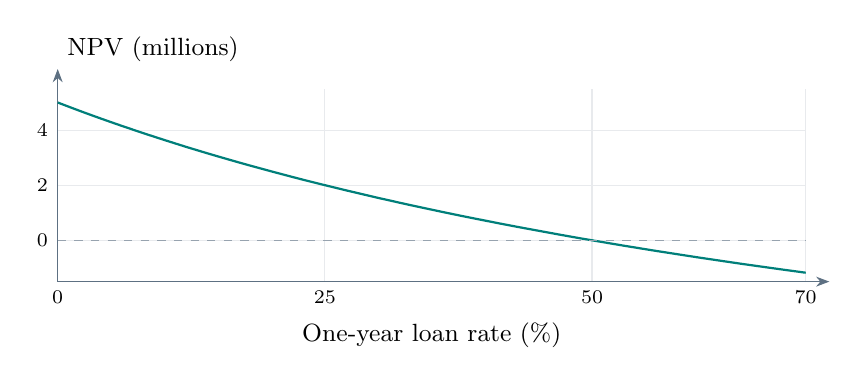
\begin{tikzpicture}[>=Stealth,every node/.style={font=\small}]
\draw[Ink!10] (0.000,0.000)--(0.000,2.450);\node[below,font=\scriptsize] at (0.000,0.000){0};
\draw[Ink!10] (3.393,0.000)--(3.393,2.450);\node[below,font=\scriptsize] at (3.393,0.000){25};
\draw[Ink!10] (6.786,0.000)--(6.786,2.450);\node[below,font=\scriptsize] at (6.786,0.000){50};
\draw[Ink!10] (9.500,0.000)--(9.500,2.450);\node[below,font=\scriptsize] at (9.500,0.000){70};
\draw[Ink!10] (0.000,0.525)--(9.500,0.525);\node[left,font=\scriptsize] at (0.000,0.525){0};
\draw[Ink!10] (0.000,1.225)--(9.500,1.225);\node[left,font=\scriptsize] at (0.000,1.225){2};
\draw[Ink!10] (0.000,1.925)--(9.500,1.925);\node[left,font=\scriptsize] at (0.000,1.925){4};
\draw[->,Ink!70] (0,0)--(9.8,0);\draw[->,Ink!70] (0,0)--(0,2.7);
\node[below] at (4.75,-.40){One-year loan rate (\%)};\node[anchor=west] at (0,2.95){NPV (millions)};
\draw[Teal,thick] plot coordinates {(0.000,2.275) (0.136,2.223) (0.271,2.172) (0.407,2.122) (0.543,2.073) (0.679,2.025) (0.814,1.978) (0.950,1.932) (1.086,1.886) (1.221,1.842) (1.357,1.798) (1.493,1.755) (1.629,1.712) (1.764,1.671) (1.900,1.630) (2.036,1.590) (2.171,1.551) (2.307,1.512) (2.443,1.474) (2.579,1.437) (2.714,1.400) (2.850,1.364) (2.986,1.328) (3.121,1.293) (3.257,1.259) (3.393,1.225) (3.529,1.192) (3.664,1.159) (3.800,1.127) (3.936,1.095) (4.071,1.063) (4.207,1.033) (4.343,1.002) (4.479,0.972) (4.614,0.943) (4.750,0.914) (4.886,0.885) (5.021,0.857) (5.157,0.829) (5.293,0.802) (5.429,0.775) (5.564,0.748) (5.700,0.722) (5.836,0.696) (5.971,0.671) (6.107,0.646) (6.243,0.621) (6.379,0.596) (6.514,0.572) (6.650,0.548) (6.786,0.525) (6.921,0.502) (7.057,0.479) (7.193,0.456) (7.329,0.434) (7.464,0.412) (7.600,0.390) (7.736,0.369) (7.871,0.348) (8.007,0.327) (8.143,0.306) (8.279,0.286) (8.414,0.266) (8.550,0.246) (8.686,0.226) (8.821,0.207) (8.957,0.188) (9.093,0.169) (9.229,0.150) (9.364,0.132) (9.500,0.113)};
\draw[Ink!45,dashed] plot coordinates {(0.000,0.525) (9.500,0.525)};

\end{tikzpicture}\end{center}\eqnote{Each project has a threshold. A collection of projects creates an investment response.}
\end{frame}

% Slide 44: IS means Investment--Saving

\begin{frame}{IS means Investment--Saving}
\point{IS lists the output/rate pairs where\par planned spending equals production.}\point{In a closed-economy equilibrium,\par planned investment equals planned national saving.}
\end{frame}

% Slide 45: Why IS slopes downward

\begin{frame}{Why IS slopes downward}
\point{A higher rate makes fewer investments worthwhile.}\point{Lower investment means less planned expenditure.}\point{Equilibrium output is lower.}\eqnote{Output is on the horizontal axis. The rate is on the vertical axis.}
\end{frame}

% Slide 46: Households respond to disposable income

\begin{frame}{Households respond to disposable income}
\[C=C_0+c(Y-T),\qquad 0<c<1.\]\begin{center}\begin{tabular}{@{}ll@{}}\toprule \textbf{Symbol} & \textbf{Meaning}\\\midrule $C$ & Planned consumption\\[2mm]
$C_0$ & Consumption independent of current income\\[2mm]
$T$ & Taxes less transfers\\[2mm]
$c$ & Extra consumption per extra unit of disposable income\\\bottomrule\end{tabular}\end{center}
\end{frame}

% Slide 47: Investment responds to the rate

\begin{frame}{Investment responds to the rate}
\[I=I_0-bi,\qquad b>0.\]\begin{center}\begin{tabular}{@{}ll@{}}\toprule \textbf{Symbol} & \textbf{Meaning}\\\midrule I & Planned investment\\[2mm]
$I_0$ & Spending independent of the current rate\\[2mm]
b & Response to the nominal rate, with other inputs fixed\\\bottomrule\end{tabular}\end{center}\eqnote{Fixed expected inflation and credit spreads make i a proxy for the relevant real financing cost.}
\end{frame}

% Slide 48: Combining spending gives the IS equation

\begin{frame}{Combining spending gives the IS equation}
\point{$G$: government consumption, fixed in this experiment.}\[Y=C+I+G.\]\[\boxed{Y=\frac{C_0-cT+I_0+G-b\nominal}{1-c}.}\]\eqnote{The equation records all goods-market equilibria for the chosen assumptions.}
\end{frame}

% Slide 49: LM means Liquidity preference--Money supply

\begin{frame}{LM means Liquidity preference--Money supply}
\point{LM lists output/rate pairs where\par desired money balances equal money supply.}\point{Holding money is useful for payments.\par Holding it also gives up interest on other assets.}
\end{frame}

% Slide 50: Why classic LM slopes upward

\begin{frame}{Why classic LM slopes upward}
\[\frac{M}{P}=L(Y,i),\qquad\frac{di}{dY}=-\frac{L_Y}{L_i}>0.\]\point{More output means more payments and a greater desire to hold money.}\point{With M/P fixed, i rises until the opportunity cost of cash offsets that extra demand.}\eqnote{The central bank chooses M. Private money demand and the bond market determine the clearing i.}
\end{frame}

% Slide 51: Agents adjust portfolios, and bond prices move

\begin{frame}{Agents adjust portfolios, and bond prices move}
\begin{center}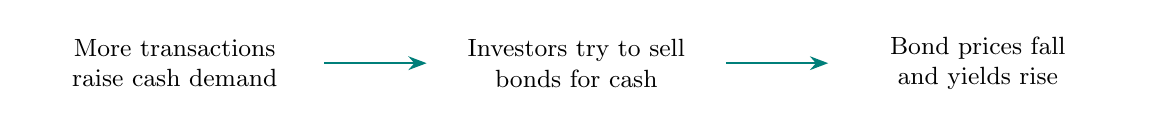
\begin{tikzpicture}[>=Stealth,every node/.style={font=\small,align=center,text width=3.5cm}]\node at (0.0,0){More transactions\\raise cash demand};\node at (5.1,0){Investors try to sell\\bonds for cash};\node at (10.2,0){Bond prices fall\\and yields rise};\draw[->,Teal,thick] (1.9,0)--(3.1999999999999997,0);\draw[->,Teal,thick] (7.0,0)--(8.299999999999999,0);\end{tikzpicture}\end{center}\point{The total money stock is unchanged. Higher i reduces desired cash holdings.}\eqnote{It is a portfolio opportunity-cost mechanism. Spending need not disappear to clear the money market.}
\end{frame}

% Slide 52: Higher output shifts money demand to the right

\begin{frame}{Higher output shifts money demand to the right}
\begin{center}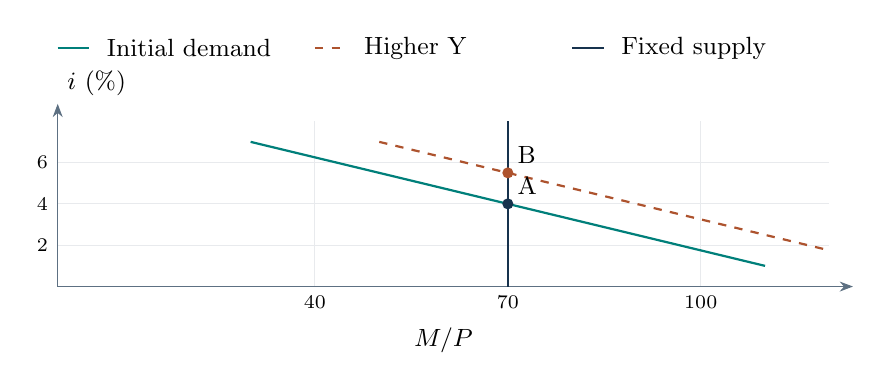
\begin{tikzpicture}[>=Stealth,every node/.style={font=\small}]
\draw[Ink!10] (3.2667,0.0000)--(3.2667,2.1000);\node[below,font=\scriptsize] at (3.2667,0.0000){40};
\draw[Ink!10] (5.7167,0.0000)--(5.7167,2.1000);\node[below,font=\scriptsize] at (5.7167,0.0000){70};
\draw[Ink!10] (8.1667,0.0000)--(8.1667,2.1000);\node[below,font=\scriptsize] at (8.1667,0.0000){100};
\draw[Ink!10] (0.0000,0.5250)--(9.8000,0.5250);\node[left,font=\scriptsize] at (0.0000,0.5250){2};
\draw[Ink!10] (0.0000,1.0500)--(9.8000,1.0500);\node[left,font=\scriptsize] at (0.0000,1.0500){4};
\draw[Ink!10] (0.0000,1.5750)--(9.8000,1.5750);\node[left,font=\scriptsize] at (0.0000,1.5750){6};
\draw[->,Ink!70] (0,0)--(10.100000000000001,0);\draw[->,Ink!70] (0,0)--(0,2.3200000000000003);
\node[below] at (4.9,-.40){$M/P$};\node[anchor=west] at (0,2.58){$i$ (\%)};
\draw[Teal,thick] plot coordinates {(2.4500,1.8375) (8.9833,0.2625)};
\draw[Rust,dashed,thick] plot coordinates {(4.0833,1.8375) (9.8000,0.4594)};
\draw[Ink,thick] plot coordinates {(5.7167,0.0000) (5.7167,2.1000)};
\fill[Ink] (5.7167,1.0500) circle (2pt);\node[above right] at (5.7167,1.0500){A};
\fill[Rust] (5.7167,1.4438) circle (2pt);\node[above right] at (5.7167,1.4438){B};
\draw[Teal,thick] (0.0,3.0300000000000002)--(0.4,3.0300000000000002);\node[anchor=west,font=\small] at (0.5,3.0300000000000002){Initial demand};
\draw[Rust,dashed] (3.266666666666667,3.0300000000000002)--(3.666666666666667,3.0300000000000002);\node[anchor=west,font=\small] at (3.766666666666667,3.0300000000000002){Higher Y};
\draw[Ink,thick] (6.533333333333334,3.0300000000000002)--(6.9333333333333345,3.0300000000000002);\node[anchor=west,font=\small] at (7.033333333333334,3.0300000000000002){Fixed supply};
\end{tikzpicture}\end{center}\eqnote{At the same fixed M/P, higher real activity raises the clearing market rate.}
\end{frame}

% Slide 53: The intersection balances both markets

\begin{frame}{The intersection balances both markets}
\begin{center}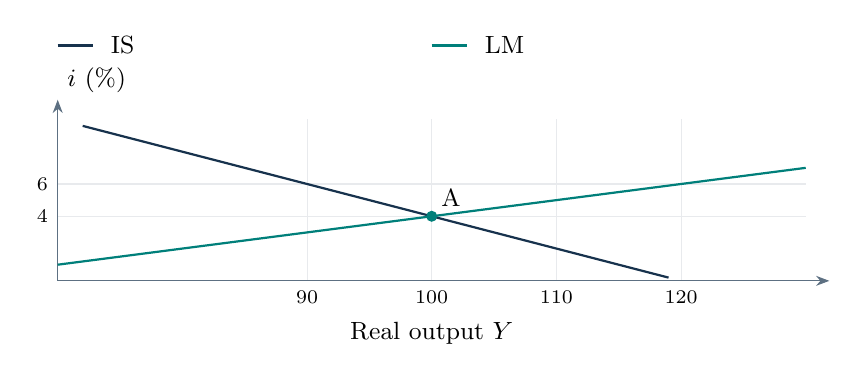
\begin{tikzpicture}[>=Stealth,every node/.style={font=\small}]
\draw[Ink!10] (3.167,0.000)--(3.167,2.050);\node[below,font=\scriptsize] at (3.167,0.000){90};
\draw[Ink!10] (4.750,0.000)--(4.750,2.050);\node[below,font=\scriptsize] at (4.750,0.000){100};
\draw[Ink!10] (6.333,0.000)--(6.333,2.050);\node[below,font=\scriptsize] at (6.333,0.000){110};
\draw[Ink!10] (7.917,0.000)--(7.917,2.050);\node[below,font=\scriptsize] at (7.917,0.000){120};
\draw[Ink!10] (0.000,0.820)--(9.500,0.820);\node[left,font=\scriptsize] at (0.000,0.820){4};
\draw[Ink!10] (0.000,1.230)--(9.500,1.230);\node[left,font=\scriptsize] at (0.000,1.230){6};
\draw[->,Ink!70] (0,0)--(9.8,0);\draw[->,Ink!70] (0,0)--(0,2.3);
\node[below] at (4.75,-.40){Real output $Y$};\node[anchor=west] at (0,2.55){$i$ (\%)};
\draw[Ink,thick] plot coordinates {(0.317,1.968) (7.758,0.041)};
\draw[Teal,thick] plot coordinates {(0.000,0.205) (9.500,1.435)};
\draw[Ink,thick] (0.0,2.9899999999999998)--(0.45,2.9899999999999998);\node[anchor=west,font=\small] at (0.55,2.9899999999999998){IS};
\draw[Teal,thick] (4.75,2.9899999999999998)--(5.2,2.9899999999999998);\node[anchor=west,font=\small] at (5.3,2.9899999999999998){LM};
\fill[Teal] (4.750,0.820) circle (2pt);\node[above right] at (4.750,0.820){A};
\end{tikzpicture}\end{center}\eqnote{At A, planned expenditure equals output and money demand equals supply.}
\end{frame}

% Slide 54: A movement along a curve versus a shift

\begin{frame}{A movement along a curve versus a shift}
\begin{center}\begin{tabular}{@{}p{.45\textwidth}p{.45\textwidth}@{}}\toprule \textbf{Movement along IS} & \textbf{A shift of IS}\\\midrule A change in the rate, holding\newline other spending inputs fixed. & A change in spending\newline at each given rate.\\\bottomrule\end{tabular}\end{center}\point{First identify what changed. Then identify which relationship changes.}
\end{frame}

% Slide 55: Monetary tightening shifts classic LM

\begin{frame}{Monetary tightening shifts classic LM}
\begin{center}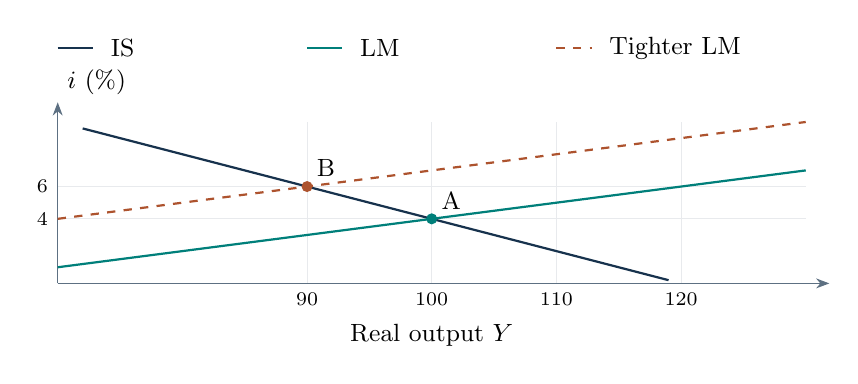
\begin{tikzpicture}[>=Stealth,every node/.style={font=\small}]
\draw[Ink!10] (3.167,0.000)--(3.167,2.050);\node[below,font=\scriptsize] at (3.167,0.000){90};
\draw[Ink!10] (4.750,0.000)--(4.750,2.050);\node[below,font=\scriptsize] at (4.750,0.000){100};
\draw[Ink!10] (6.333,0.000)--(6.333,2.050);\node[below,font=\scriptsize] at (6.333,0.000){110};
\draw[Ink!10] (7.917,0.000)--(7.917,2.050);\node[below,font=\scriptsize] at (7.917,0.000){120};
\draw[Ink!10] (0.000,0.820)--(9.500,0.820);\node[left,font=\scriptsize] at (0.000,0.820){4};
\draw[Ink!10] (0.000,1.230)--(9.500,1.230);\node[left,font=\scriptsize] at (0.000,1.230){6};
\draw[->,Ink!70] (0,0)--(9.8,0);\draw[->,Ink!70] (0,0)--(0,2.3);
\node[below] at (4.75,-.40){Real output $Y$};\node[anchor=west] at (0,2.55){$i$ (\%)};
\draw[Ink,thick] plot coordinates {(0.317,1.968) (7.758,0.041)};
\draw[Teal,thick] plot coordinates {(0.000,0.205) (9.500,1.435)};
\draw[Rust,thick,dashed] plot coordinates {(0.000,0.820) (9.500,2.050)};
\draw[Ink,thick] (0.0,2.9899999999999998)--(0.45,2.9899999999999998);\node[anchor=west,font=\small] at (0.55,2.9899999999999998){IS};
\draw[Teal,thick] (3.1666666666666665,2.9899999999999998)--(3.6166666666666667,2.9899999999999998);\node[anchor=west,font=\small] at (3.716666666666667,2.9899999999999998){LM};
\draw[Rust,thick,dashed] (6.333333333333333,2.9899999999999998)--(6.783333333333333,2.9899999999999998);\node[anchor=west,font=\small] at (6.883333333333333,2.9899999999999998){Tighter LM};
\fill[Teal] (4.750,0.820) circle (2pt);\node[above right] at (4.750,0.820){A};\fill[Rust] (3.167,1.230) circle (2pt);\node[above right] at (3.167,1.230){B};
\end{tikzpicture}\end{center}\eqnote{Lower real money supply: A becomes B. The rate rises and output falls.}
\end{frame}

% Slide 56: Fiscal expansion with an unchanged money supply

\begin{frame}{Fiscal expansion with an unchanged money supply}
\begin{center}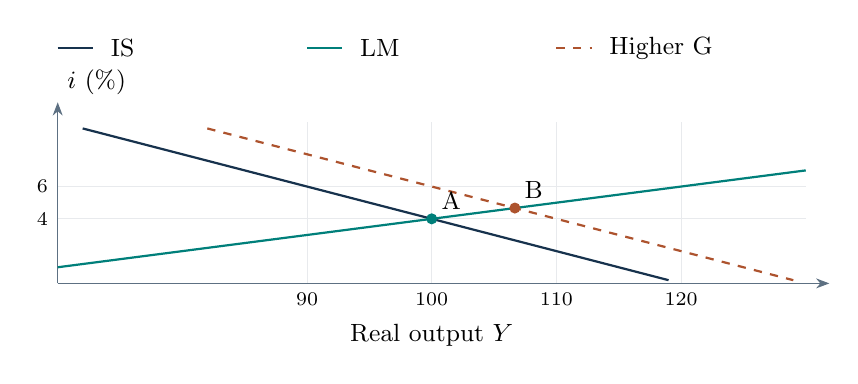
\begin{tikzpicture}[>=Stealth,every node/.style={font=\small}]
\draw[Ink!10] (3.167,0.000)--(3.167,2.050);\node[below,font=\scriptsize] at (3.167,0.000){90};
\draw[Ink!10] (4.750,0.000)--(4.750,2.050);\node[below,font=\scriptsize] at (4.750,0.000){100};
\draw[Ink!10] (6.333,0.000)--(6.333,2.050);\node[below,font=\scriptsize] at (6.333,0.000){110};
\draw[Ink!10] (7.917,0.000)--(7.917,2.050);\node[below,font=\scriptsize] at (7.917,0.000){120};
\draw[Ink!10] (0.000,0.820)--(9.500,0.820);\node[left,font=\scriptsize] at (0.000,0.820){4};
\draw[Ink!10] (0.000,1.230)--(9.500,1.230);\node[left,font=\scriptsize] at (0.000,1.230){6};
\draw[->,Ink!70] (0,0)--(9.8,0);\draw[->,Ink!70] (0,0)--(0,2.3);
\node[below] at (4.75,-.40){Real output $Y$};\node[anchor=west] at (0,2.55){$i$ (\%)};
\draw[Ink,thick] plot coordinates {(0.317,1.968) (7.758,0.041)};
\draw[Teal,thick] plot coordinates {(0.000,0.205) (9.500,1.435)};
\draw[Rust,thick,dashed] plot coordinates {(1.900,1.968) (9.342,0.041)};
\draw[Ink,thick] (0.0,2.9899999999999998)--(0.45,2.9899999999999998);\node[anchor=west,font=\small] at (0.55,2.9899999999999998){IS};
\draw[Teal,thick] (3.1666666666666665,2.9899999999999998)--(3.6166666666666667,2.9899999999999998);\node[anchor=west,font=\small] at (3.716666666666667,2.9899999999999998){LM};
\draw[Rust,thick,dashed] (6.333333333333333,2.9899999999999998)--(6.783333333333333,2.9899999999999998);\node[anchor=west,font=\small] at (6.883333333333333,2.9899999999999998){Higher G};
\fill[Teal] (4.750,0.820) circle (2pt);\node[above right] at (4.750,0.820){A};\fill[Rust] (5.806,0.957) circle (2pt);\node[above right] at (5.806,0.957){B};
\end{tikzpicture}\end{center}\eqnote{The same IS shift raises output and the rate. Private investment partly falls.}
\end{frame}

% Slide 57: A demand shock versus a supply shock

\begin{frame}{A demand shock versus a supply shock}
\point{Lower confidence shifts planned spending inward.}\point{Lower productive capacity moves potential output.}\point{Policy faces different inflation consequences in the two cases.}
\end{frame}

% Slide 58: Inflation and policy feedback
\section[Inflation and policy feedback]{Inflation and policy feedback}
\begin{frame}[plain]
{\color{Gold}\large LECTURE 2}\par\vspace{9mm}{\Huge\bfseries Inflation and policy feedback}\par\vspace{7mm}{\Large Why can a central bank raise nominal rates by more than inflation?}
\end{frame}

% Slide 59: The neutral real rate is a benchmark

\begin{frame}{The neutral real rate is a benchmark}
\point{$\neutral$: the real rate consistent with output\par at potential and stable inflation.}\point{The actual real rate may be above or below it.}\eqnote{Neutral is an estimate. It depends on the economy\textquotesingle s resources, preferences and opportunities.}
\end{frame}

% Slide 60: At the target, a neutral nominal benchmark

\begin{frame}{At the target, a neutral nominal benchmark}
\[\policy\approx\neutral+\pi^*.\]\point{$\pi^*$: the inflation target.}\[\neutral=1\%,\quad\pi^*=2\%\quad\Rightarrow\quad\policy\approx3\%.\]
\end{frame}

% Slide 61: If inflation rises, the nominal rate must catch up

\begin{frame}{If inflation rises, the nominal rate must catch up}
\point{Suppose actual and expected inflation rise from 2\% to 3\%.}\[\text{To keep a 1\% real rate:}\quad\policy=4\%.\]\point{To add restraint, an illustrative rule raises it further to 4.5\%.}
\end{frame}

% Slide 62: US inflation and policy after Covid

\begin{frame}{US inflation and policy after Covid}
\begin{center}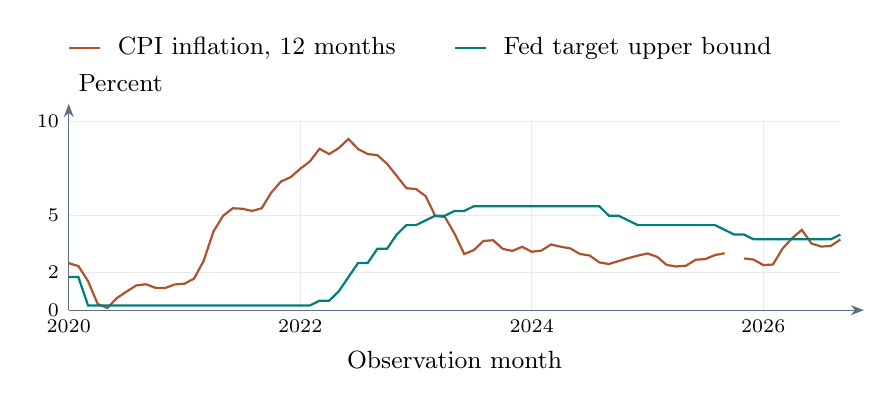
\begin{tikzpicture}[>=Stealth,every node/.style={font=\small}]
\draw[Ink!10] (0.0000,0.0000)--(0.0000,2.4000);\node[below,font=\scriptsize] at (0.0000,0.0000){2020};
\draw[Ink!10] (2.9400,0.0000)--(2.9400,2.4000);\node[below,font=\scriptsize] at (2.9400,0.0000){2022};
\draw[Ink!10] (5.8800,0.0000)--(5.8800,2.4000);\node[below,font=\scriptsize] at (5.8800,0.0000){2024};
\draw[Ink!10] (8.8200,0.0000)--(8.8200,2.4000);\node[below,font=\scriptsize] at (8.8200,0.0000){2026};
\draw[Ink!10] (0.0000,0.0000)--(9.8000,0.0000);\node[left,font=\scriptsize] at (0.0000,0.0000){0};
\draw[Ink!10] (0.0000,0.4800)--(9.8000,0.4800);\node[left,font=\scriptsize] at (0.0000,0.4800){2};
\draw[Ink!10] (0.0000,1.2000)--(9.8000,1.2000);\node[left,font=\scriptsize] at (0.0000,1.2000){5};
\draw[Ink!10] (0.0000,2.4000)--(9.8000,2.4000);\node[left,font=\scriptsize] at (0.0000,2.4000){10};
\draw[->,Ink!70] (0,0)--(10.100000000000001,0);\draw[->,Ink!70] (0,0)--(0,2.62);
\node[below] at (4.9,-.40){Observation month};\node[anchor=west] at (0,2.88){Percent};
\draw[Rust,thick] plot coordinates {(0.0000,0.5968) (0.1225,0.5604) (0.2450,0.3694) (0.3675,0.0790) (0.4900,0.0283) (0.6125,0.1550) (0.7350,0.2367) (0.8575,0.3143) (0.9800,0.3291) (1.1025,0.2837) (1.2250,0.2819) (1.3475,0.3269) (1.4700,0.3359) (1.5925,0.4023) (1.7150,0.6287) (1.8375,0.9983) (1.9600,1.1982) (2.0825,1.2939) (2.2050,1.2877) (2.3275,1.2603) (2.4500,1.2937) (2.5725,1.4932) (2.6950,1.6342) (2.8175,1.6887) (2.9400,1.7952) (3.0625,1.8891) (3.1850,2.0502) (3.3075,1.9821) (3.4300,2.0596) (3.5525,2.1743) (3.6750,2.0460) (3.7975,1.9830) (3.9200,1.9684) (4.0425,1.8589) (4.1650,1.7065) (4.2875,1.5491) (4.4100,1.5384) (4.5325,1.4485) (4.6550,1.1964) (4.7775,1.1833) (4.9000,0.9714) (5.0225,0.7126) (5.1450,0.7627) (5.2675,0.8796) (5.3900,0.8879) (5.5125,0.7779) (5.6350,0.7529) (5.7575,0.8045) (5.8800,0.7418) (6.0025,0.7568) (6.1250,0.8346) (6.2475,0.8058) (6.3700,0.7846) (6.4925,0.7131) (6.6150,0.6947) (6.7375,0.6074) (6.8600,0.5858) (6.9825,0.6235) (7.1050,0.6599) (7.2275,0.6931) (7.3500,0.7201) (7.4725,0.6772) (7.5950,0.5738) (7.7175,0.5547) (7.8400,0.5652) (7.9625,0.6406) (8.0850,0.6492) (8.2075,0.6999) (8.3300,0.7230)};
\draw[Rust,thick] plot coordinates {(8.5750,0.6564) (8.6975,0.6425) (8.8200,0.5727) (8.9425,0.5794) (9.0650,0.7815) (9.1875,0.9146) (9.3100,1.0197) (9.4325,0.8475) (9.5550,0.8076) (9.6775,0.8152) (9.8000,0.8970)};
\draw[Teal,thick] plot coordinates {(0.0000,0.4200) (0.1225,0.4200) (0.2450,0.0600) (0.3675,0.0600) (0.4900,0.0600) (0.6125,0.0600) (0.7350,0.0600) (0.8575,0.0600) (0.9800,0.0600) (1.1025,0.0600) (1.2250,0.0600) (1.3475,0.0600) (1.4700,0.0600) (1.5925,0.0600) (1.7150,0.0600) (1.8375,0.0600) (1.9600,0.0600) (2.0825,0.0600) (2.2050,0.0600) (2.3275,0.0600) (2.4500,0.0600) (2.5725,0.0600) (2.6950,0.0600) (2.8175,0.0600) (2.9400,0.0600) (3.0625,0.0600) (3.1850,0.1200) (3.3075,0.1200) (3.4300,0.2400) (3.5525,0.4200) (3.6750,0.6000) (3.7975,0.6000) (3.9200,0.7800) (4.0425,0.7800) (4.1650,0.9600) (4.2875,1.0800) (4.4100,1.0800) (4.5325,1.1400) (4.6550,1.2000) (4.7775,1.2000) (4.9000,1.2600) (5.0225,1.2600) (5.1450,1.3200) (5.2675,1.3200) (5.3900,1.3200) (5.5125,1.3200) (5.6350,1.3200) (5.7575,1.3200) (5.8800,1.3200) (6.0025,1.3200) (6.1250,1.3200) (6.2475,1.3200) (6.3700,1.3200) (6.4925,1.3200) (6.6150,1.3200) (6.7375,1.3200) (6.8600,1.2000) (6.9825,1.2000) (7.1050,1.1400) (7.2275,1.0800) (7.3500,1.0800) (7.4725,1.0800) (7.5950,1.0800) (7.7175,1.0800) (7.8400,1.0800) (7.9625,1.0800) (8.0850,1.0800) (8.2075,1.0800) (8.3300,1.0200) (8.4525,0.9600) (8.5750,0.9600) (8.6975,0.9000) (8.8200,0.9000) (8.9425,0.9000) (9.0650,0.9000) (9.1875,0.9000) (9.3100,0.9000) (9.4325,0.9000) (9.5550,0.9000) (9.6775,0.9000) (9.8000,0.9600)};
\draw[Rust,thick] (0.0,3.33)--(0.4,3.33);\node[anchor=west,font=\small] at (0.5,3.33){CPI inflation, 12 months};
\draw[Teal,thick] (4.9,3.33)--(5.300000000000001,3.33);\node[anchor=west,font=\small] at (5.4,3.33){Fed target upper bound};
\end{tikzpicture}\end{center}\eqnote{Jan 2020–Sep 2026. BLS/Federal Reserve via FRED. Policy: month-end. Missing Oct 2025 CPI is a gap.}
\end{frame}

% Slide 63: The output gap measures pressure on resources

\begin{frame}{The output gap measures pressure on resources}
\[x_t=100\frac{Y_t-Y_t^*}{Y_t^*}.\]\begin{center}\begin{tabular}{@{}ll@{}}\toprule \textbf{Symbol} & \textbf{Meaning}\\\midrule $Y_t$ & Actual real output\\[2mm]
$Y_t^*$ & Potential real output\\[2mm]
$x_t$ & Output gap in percent\\\bottomrule\end{tabular}\end{center}\eqnote{Positive gap: output above potential. Negative gap: slack.}
\end{frame}

% Slide 64: Weak activity changes the policy trade-off

\begin{frame}{Weak activity changes the policy trade-off}
\point{Keep inflation at 3\%, but put output 2\% below potential.}\[\text{Illustrative response:}\quad4.5-0.5\times2=3.5\%.\]\point{Inflation calls for restraint. Slack calls for support.}
\end{frame}

% Slide 65: A central banker might follow a rule like this

\begin{frame}{A central banker might follow a rule like this}
\[\boxed{\bar i_t=r^*+\pi_t+0.5(\pi_t-\pi^*)+0.5x_t.}\]\point{One possible policy reaction: respond to inflation and the output gap.}\eqnote{Illustrative Taylor-style rule. Rates and gaps use percentage points; this is not a commitment.}
\end{frame}

% Slide 66: A simple Phillips relationship

\begin{frame}{A simple Phillips relationship}
\[\pi_t=\pi_t^e+\kappa x_t+u_t.\]\begin{center}\begin{tabular}{@{}ll@{}}\toprule \textbf{Symbol} & \textbf{Meaning}\\\midrule $\pi_t^e$ & Expected inflation for this period\\[2mm]
$x_t$ & Output gap, as defined earlier\\[2mm]
$\kappa>0$ & Inflation response to demand pressure\\[2mm]
$u_t$ & Cost or supply disturbance\\\bottomrule\end{tabular}\end{center}
\end{frame}

% Slide 67: Expectations shift the Phillips curve

\begin{frame}{Expectations shift the Phillips curve}
\begin{center}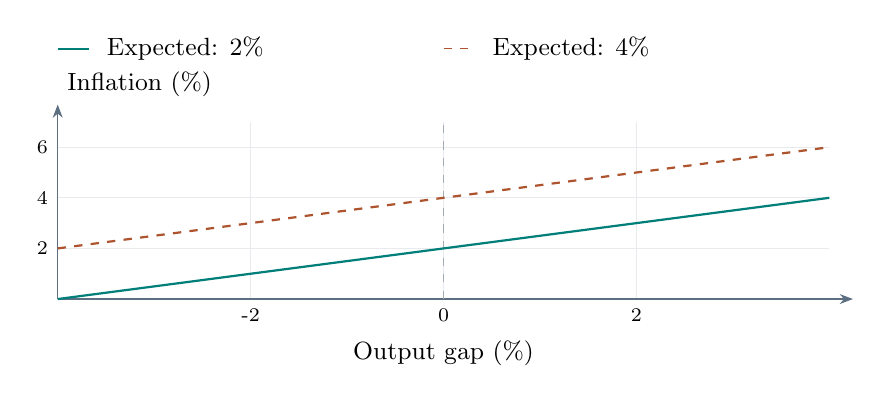
\begin{tikzpicture}[>=Stealth,every node/.style={font=\small}]
\draw[Ink!10] (2.4500,0.0000)--(2.4500,2.2500);\node[below,font=\scriptsize] at (2.4500,0.0000){-2};
\draw[Ink!10] (4.9000,0.0000)--(4.9000,2.2500);\node[below,font=\scriptsize] at (4.9000,0.0000){0};
\draw[Ink!10] (7.3500,0.0000)--(7.3500,2.2500);\node[below,font=\scriptsize] at (7.3500,0.0000){2};
\draw[Ink!10] (0.0000,0.6429)--(9.8000,0.6429);\node[left,font=\scriptsize] at (0.0000,0.6429){2};
\draw[Ink!10] (0.0000,1.2857)--(9.8000,1.2857);\node[left,font=\scriptsize] at (0.0000,1.2857){4};
\draw[Ink!10] (0.0000,1.9286)--(9.8000,1.9286);\node[left,font=\scriptsize] at (0.0000,1.9286){6};
\draw[->,Ink!70] (0,0)--(10.100000000000001,0);\draw[->,Ink!70] (0,0)--(0,2.47);
\node[below] at (4.9,-.40){Output gap (\%)};\node[anchor=west] at (0,2.73){Inflation (\%)};
\draw[Ink!40,dashed] (4.9000,0.0000)--(4.9000,2.2500);
\draw[Teal,thick] plot coordinates {(0.0000,0.0000) (9.8000,1.2857)};
\draw[Rust,thick,dashed] plot coordinates {(0.0000,0.6429) (9.8000,1.9286)};
\draw[Teal,thick] (0.0,3.18)--(0.4,3.18);\node[anchor=west,font=\small] at (0.5,3.18){Expected: 2\%};
\draw[Rust,dashed] (4.9,3.18)--(5.300000000000001,3.18);\node[anchor=west,font=\small] at (5.4,3.18){Expected: 4\%};
\end{tikzpicture}\end{center}\eqnote{Hypothetical $\kappa=0.5$ and no supply disturbance.}
\end{frame}

% Slide 68: Inflation deviations are easier to analyse

\begin{frame}{Inflation deviations are easier to analyse}
\[d_t=\pi_t-\pi^*.\]\begin{center}\begin{tabular}{@{}ll@{}}\toprule \textbf{Symbol} & \textbf{Meaning}\\\midrule $d_t$ & Inflation deviation from target, in percentage points\\[2mm]
$\pi_t$ & Inflation rate\\[2mm]
$\pi^*$ & Inflation target\\\bottomrule\end{tabular}\end{center}\point{Inflation of 3\% with a 2\% target means $d_t=1$.}
\end{frame}

% Slide 69: A simple model of inflation persistence

\begin{frame}{A simple model of inflation persistence}
\[d_t=a\,d_{t-1}+u_t.\]\begin{center}\begin{tabular}{@{}ll@{}}\toprule \textbf{Symbol} & \textbf{Meaning}\\\midrule $a$ & Net carry-over from the previous inflation deviation\\[2mm]
$u_t$ & A new inflation disturbance this period\\\bottomrule\end{tabular}\end{center}\eqnote{After an initial shock, set later disturbances to zero and compare values of a.}
\end{frame}

% Slide 70: The same shock can decay or amplify

\begin{frame}{The same shock can decay or amplify}
\begin{center}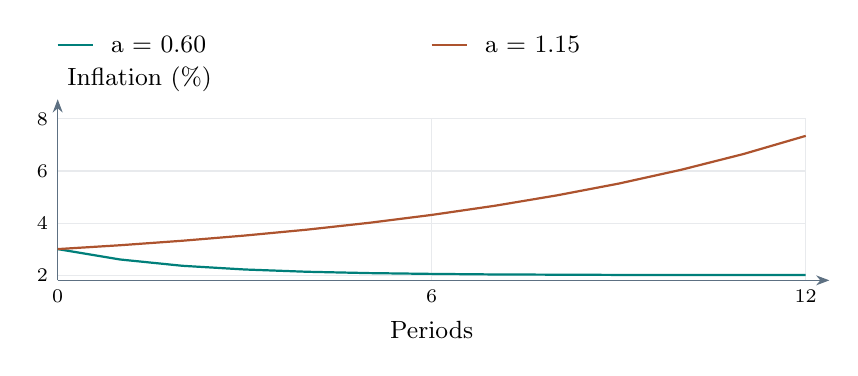
\begin{tikzpicture}[>=Stealth,every node/.style={font=\small}]
\draw[Ink!10] (0.000,0.000)--(0.000,2.050);\node[below,font=\scriptsize] at (0.000,0.000){0};
\draw[Ink!10] (4.750,0.000)--(4.750,2.050);\node[below,font=\scriptsize] at (4.750,0.000){6};
\draw[Ink!10] (9.500,0.000)--(9.500,2.050);\node[below,font=\scriptsize] at (9.500,0.000){12};
\draw[Ink!10] (0.000,0.066)--(9.500,0.066);\node[left,font=\scriptsize] at (0.000,0.066){2};
\draw[Ink!10] (0.000,0.727)--(9.500,0.727);\node[left,font=\scriptsize] at (0.000,0.727){4};
\draw[Ink!10] (0.000,1.389)--(9.500,1.389);\node[left,font=\scriptsize] at (0.000,1.389){6};
\draw[Ink!10] (0.000,2.050)--(9.500,2.050);\node[left,font=\scriptsize] at (0.000,2.050){8};
\draw[->,Ink!70] (0,0)--(9.8,0);\draw[->,Ink!70] (0,0)--(0,2.3);
\node[below] at (4.75,-.40){Periods};\node[anchor=west] at (0,2.55){Inflation (\%)};
\draw[Teal,thick] plot coordinates {(0.000,0.397) (0.792,0.265) (1.583,0.185) (2.375,0.138) (3.167,0.109) (3.958,0.092) (4.750,0.082) (5.542,0.075) (6.333,0.072) (7.125,0.069) (7.917,0.068) (8.708,0.067) (9.500,0.067)};
\draw[Rust,thick] plot coordinates {(0.000,0.397) (0.792,0.446) (1.583,0.503) (2.375,0.569) (3.167,0.644) (3.958,0.731) (4.750,0.831) (5.542,0.946) (6.333,1.078) (7.125,1.229) (7.917,1.404) (8.708,1.604) (9.500,1.835)};
\draw[Teal,thick] (0.0,2.9899999999999998)--(0.45,2.9899999999999998);\node[anchor=west,font=\small] at (0.55,2.9899999999999998){a = 0.60};
\draw[Rust,thick] (4.75,2.9899999999999998)--(5.2,2.9899999999999998);\node[anchor=west,font=\small] at (5.3,2.9899999999999998){a = 1.15};

\end{tikzpicture}\end{center}\eqnote{Target 2\%, initial deviation 1 point. Stable when $|a|<1$. Original hypothetical paths.}
\end{frame}

% Slide 71: Exercise: inflation rises while output falls

\begin{frame}{Exercise: inflation rises while output falls}
\point{An energy shortage raises costs and reduces productive capacity.}\point{Compare holding the nominal rate fixed with raising it.}\point{Which assumptions determine the change in the real rate?}
\end{frame}

% Slide 72: Modern rate targeting
\section[Modern rate targeting]{Modern rate targeting}
\begin{frame}[plain]
{\color{Gold}\large LECTURE 2}\par\vspace{9mm}{\Huge\bfseries Modern rate targeting}\par\vspace{7mm}{\Large What changes when the central bank chooses the rate?}
\end{frame}

% Slide 73: Choose the rate, and let the monetary quantity adjust

\begin{frame}{Choose the rate, and let the monetary quantity adjust}
\[i=\bar i,\qquad\frac{M}{P}=L(Y,\bar i).\]\point{The central bank chooses the target. It accommodates the quantity needed to implement it.}\point{For this experiment, the target is fixed as Y changes.}\eqnote{Across meetings, the chosen target can respond to inflation and activity.}
\end{frame}

% Slide 74: With a rate target, policy sets a horizontal line

\begin{frame}{With a rate target, policy sets a horizontal line}
\begin{center}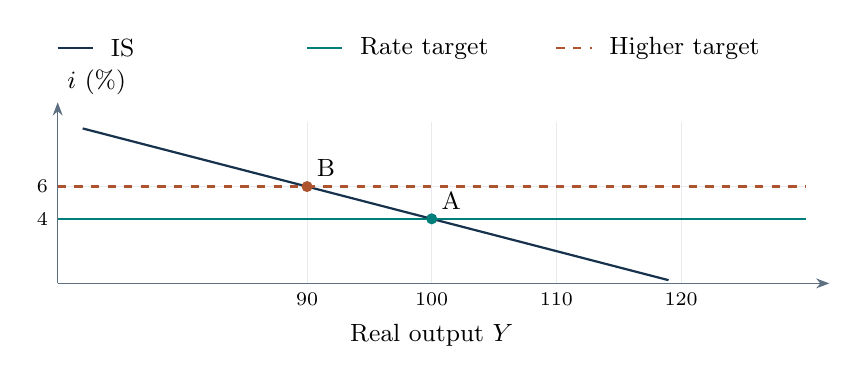
\begin{tikzpicture}[>=Stealth,every node/.style={font=\small}]
\draw[Ink!10] (3.167,0.000)--(3.167,2.050);\node[below,font=\scriptsize] at (3.167,0.000){90};
\draw[Ink!10] (4.750,0.000)--(4.750,2.050);\node[below,font=\scriptsize] at (4.750,0.000){100};
\draw[Ink!10] (6.333,0.000)--(6.333,2.050);\node[below,font=\scriptsize] at (6.333,0.000){110};
\draw[Ink!10] (7.917,0.000)--(7.917,2.050);\node[below,font=\scriptsize] at (7.917,0.000){120};
\draw[Ink!10] (0.000,0.820)--(9.500,0.820);\node[left,font=\scriptsize] at (0.000,0.820){4};
\draw[Ink!10] (0.000,1.230)--(9.500,1.230);\node[left,font=\scriptsize] at (0.000,1.230){6};
\draw[->,Ink!70] (0,0)--(9.8,0);\draw[->,Ink!70] (0,0)--(0,2.3);
\node[below] at (4.75,-.40){Real output $Y$};\node[anchor=west] at (0,2.55){$i$ (\%)};
\draw[Ink,thick] plot coordinates {(0.317,1.968) (7.758,0.041)};
\draw[Teal,thick] plot coordinates {(0.000,0.820) (9.500,0.820)};
\draw[Rust,thick,dashed] plot coordinates {(0.000,1.230) (9.500,1.230)};
\draw[Ink,thick] (0.0,2.9899999999999998)--(0.45,2.9899999999999998);\node[anchor=west,font=\small] at (0.55,2.9899999999999998){IS};
\draw[Teal,thick] (3.1666666666666665,2.9899999999999998)--(3.6166666666666667,2.9899999999999998);\node[anchor=west,font=\small] at (3.716666666666667,2.9899999999999998){Rate target};
\draw[Rust,thick,dashed] (6.333333333333333,2.9899999999999998)--(6.783333333333333,2.9899999999999998);\node[anchor=west,font=\small] at (6.883333333333333,2.9899999999999998){Higher target};
\fill[Teal] (4.750,0.820) circle (2pt);\node[above right] at (4.750,0.820){A};\fill[Rust] (3.167,1.230) circle (2pt);\node[above right] at (3.167,1.230){B};
\end{tikzpicture}\end{center}\eqnote{Chosen $i=\bar i$ rises from 4\% to 6\%; output falls from 100 to 90.}
\end{frame}

% Slide 75: Fiscal expansion with an unchanged rate target

\begin{frame}{Fiscal expansion with an unchanged rate target}
\begin{center}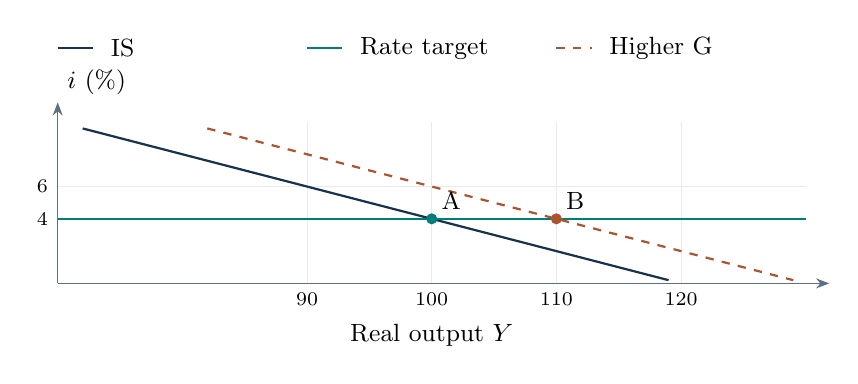
\begin{tikzpicture}[>=Stealth,every node/.style={font=\small}]
\draw[Ink!10] (3.167,0.000)--(3.167,2.050);\node[below,font=\scriptsize] at (3.167,0.000){90};
\draw[Ink!10] (4.750,0.000)--(4.750,2.050);\node[below,font=\scriptsize] at (4.750,0.000){100};
\draw[Ink!10] (6.333,0.000)--(6.333,2.050);\node[below,font=\scriptsize] at (6.333,0.000){110};
\draw[Ink!10] (7.917,0.000)--(7.917,2.050);\node[below,font=\scriptsize] at (7.917,0.000){120};
\draw[Ink!10] (0.000,0.820)--(9.500,0.820);\node[left,font=\scriptsize] at (0.000,0.820){4};
\draw[Ink!10] (0.000,1.230)--(9.500,1.230);\node[left,font=\scriptsize] at (0.000,1.230){6};
\draw[->,Ink!70] (0,0)--(9.8,0);\draw[->,Ink!70] (0,0)--(0,2.3);
\node[below] at (4.75,-.40){Real output $Y$};\node[anchor=west] at (0,2.55){$i$ (\%)};
\draw[Ink,thick] plot coordinates {(0.317,1.968) (7.758,0.041)};
\draw[Teal,thick] plot coordinates {(0.000,0.820) (9.500,0.820)};
\draw[Rust,thick,dashed] plot coordinates {(1.900,1.968) (9.342,0.041)};
\draw[Ink,thick] (0.0,2.9899999999999998)--(0.45,2.9899999999999998);\node[anchor=west,font=\small] at (0.55,2.9899999999999998){IS};
\draw[Teal,thick] (3.1666666666666665,2.9899999999999998)--(3.6166666666666667,2.9899999999999998);\node[anchor=west,font=\small] at (3.716666666666667,2.9899999999999998){Rate target};
\draw[Rust,thick,dashed] (6.333333333333333,2.9899999999999998)--(6.783333333333333,2.9899999999999998);\node[anchor=west,font=\small] at (6.883333333333333,2.9899999999999998){Higher G};
\fill[Teal] (4.750,0.820) circle (2pt);\node[above right] at (4.750,0.820){A};\fill[Rust] (6.333,0.820) circle (2pt);\node[above right] at (6.333,0.820){B};
\end{tikzpicture}\end{center}\eqnote{Higher government spending shifts IS outward. At a fixed rate, output rises.}
\end{frame}

% Slide 76: A private-demand slowdown shifts IS inward

\begin{frame}{A private-demand slowdown shifts IS inward}
\begin{center}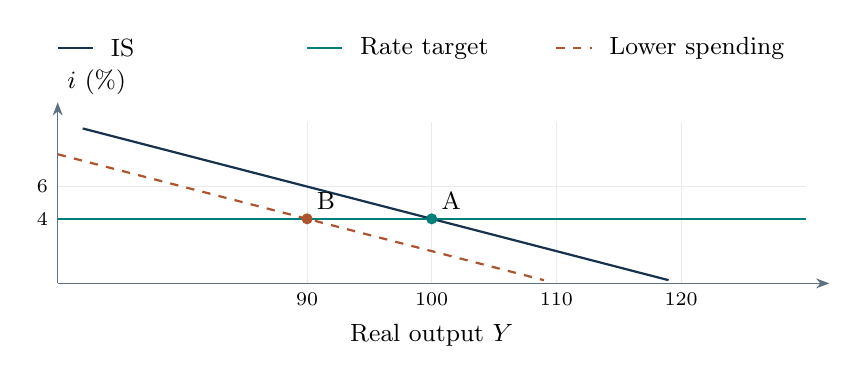
\begin{tikzpicture}[>=Stealth,every node/.style={font=\small}]
\draw[Ink!10] (3.167,0.000)--(3.167,2.050);\node[below,font=\scriptsize] at (3.167,0.000){90};
\draw[Ink!10] (4.750,0.000)--(4.750,2.050);\node[below,font=\scriptsize] at (4.750,0.000){100};
\draw[Ink!10] (6.333,0.000)--(6.333,2.050);\node[below,font=\scriptsize] at (6.333,0.000){110};
\draw[Ink!10] (7.917,0.000)--(7.917,2.050);\node[below,font=\scriptsize] at (7.917,0.000){120};
\draw[Ink!10] (0.000,0.820)--(9.500,0.820);\node[left,font=\scriptsize] at (0.000,0.820){4};
\draw[Ink!10] (0.000,1.230)--(9.500,1.230);\node[left,font=\scriptsize] at (0.000,1.230){6};
\draw[->,Ink!70] (0,0)--(9.8,0);\draw[->,Ink!70] (0,0)--(0,2.3);
\node[below] at (4.75,-.40){Real output $Y$};\node[anchor=west] at (0,2.55){$i$ (\%)};
\draw[Ink,thick] plot coordinates {(0.317,1.968) (7.758,0.041)};
\draw[Teal,thick] plot coordinates {(0.000,0.820) (9.500,0.820)};
\draw[Rust,thick,dashed] plot coordinates {(0.000,1.640) (6.175,0.041)};
\draw[Ink,thick] (0.0,2.9899999999999998)--(0.45,2.9899999999999998);\node[anchor=west,font=\small] at (0.55,2.9899999999999998){IS};
\draw[Teal,thick] (3.1666666666666665,2.9899999999999998)--(3.6166666666666667,2.9899999999999998);\node[anchor=west,font=\small] at (3.716666666666667,2.9899999999999998){Rate target};
\draw[Rust,thick,dashed] (6.333333333333333,2.9899999999999998)--(6.783333333333333,2.9899999999999998);\node[anchor=west,font=\small] at (6.883333333333333,2.9899999999999998){Lower spending};
\fill[Teal] (4.750,0.820) circle (2pt);\node[above right] at (4.750,0.820){A};\fill[Rust] (3.167,0.820) circle (2pt);\node[above right] at (3.167,0.820){B};
\end{tikzpicture}\end{center}\eqnote{Lower autonomous consumption or investment reduces output at a fixed target.}
\end{frame}

% Slide 77: Optional mathematical extension
\section[Optional mathematical extension]{Optional mathematical extension}
\begin{frame}[plain]
{\color{Gold}\large LECTURE 2}\par\vspace{9mm}{\Huge\bfseries Optional mathematical extension}\par\vspace{7mm}{\Large How does policy change an inflation recurrence?}
\end{frame}

% Slide 78: Optional extension: what changes the feedback?

\begin{frame}{Optional extension: what changes the feedback?}
\point{We will connect three mechanisms:}\point{Inflation pressure, the demand response to real rates,\par and a policy response to inflation.}\eqnote{Each relationship comes next on its own slide. The coefficients describe this toy model only.}
\end{frame}

% Slide 79: Inflation responds to activity and past inflation

\begin{frame}{Inflation responds to activity and past inflation}
\[d_t=\alpha d_{t-1}+\kappa x_t+u_t.\]\begin{center}\begin{tabular}{@{}ll@{}}\toprule \textbf{New coefficient} & \textbf{Meaning}\\\midrule $\alpha$ & Carry-over of the previous inflation deviation\\[2mm]
$\kappa>0$ & Inflation response to a one-point output gap\\\bottomrule\end{tabular}\end{center}\eqnote{d is the inflation deviation, x the output gap, and u a new disturbance.}
\end{frame}

% Slide 80: Real-rate restraint reduces the output gap

\begin{frame}{Real-rate restraint reduces the output gap}
\[x_t=-B(\realrate_t-\neutral),\qquad B>0.\]\point{$B$: how strongly demand responds to the real-rate gap.}\eqnote{Higher real rates relative to neutral reduce demand.\par B is an aggregate sensitivity, distinct from investment\textquotesingle s earlier coefficient b.}
\end{frame}

% Slide 81: Policy adds real restraint when inflation exceeds target

\begin{frame}{Policy adds real restraint when inflation exceeds target}
\[\realrate_t-\neutral=\phi d_{t-1},\qquad\phi>0.\]\point{$\phi$: the real-rate response to a one-point inflation deviation.}\eqnote{The nominal policy rate must also offset expected inflation to deliver this real response.}
\end{frame}

% Slide 82: Substitution gives a stability condition

\begin{frame}{Substitution gives a stability condition}
\[d_t=\underbrace{(\alpha-\kappa B\phi)}_{a}\,d_{t-1}+u_t.\]\[\boxed{|\alpha-\kappa B\phi|<1.}\]\point{If $\alpha=1.15$ and $\kappa B\phi=0.55$, then $a=0.60$.}\eqnote{Policy supplies negative feedback in this specified model.}
\end{frame}

% Slide 83: A two-date endowment economy

\begin{frame}{A two-date endowment economy}
\[U=\ln c_0+\beta\ln c_1.\]\point{$c_0,c_1$: consumption now and later. $\beta>0$: patience.}\point{$e_0,e_1$: the economy’s available resources on the two dates.}\eqnote{$U$: lifetime utility. The real bond transfers purchasing power between dates.}
\end{frame}

% Slide 84: The individual intertemporal budget

\begin{frame}{The individual intertemporal budget}
\[c_0+\frac{c_1}{1+\realrate}=e_0+\frac{e_1}{1+\realrate}.\]\point{Saving one unit now buys a claim to future resources.}\point{The individual chooses consumption given the rate.}
\end{frame}

% Slide 85: Market clearing pins down a real rate

\begin{frame}{Market clearing pins down a real rate}
\[\frac1{c_0}=\beta(1+\realrate)\frac1{c_1},\qquad c_0=e_0,\quad c_1=e_1.\]\[\boxed{1+\realrate=\frac{e_1}{\beta e_0}.}\]\point{More resources now lower the rate, other inputs fixed.}
\end{frame}

% Slide 86: Further reading
\section[Reading]{Reading}
\begin{frame}{Further reading}
\point{Dmitriy Sergeyev, Bocconi 30054 course materials.}\point{Krugman, Obstfeld \& Melitz, \emph{International Economics}.}\point{Source links and worked answers accompany each slide in the notes.}
\end{frame}
\end{document}
